\documentclass{article}
\usepackage{graphicx}
\usepackage{tikz}
\usepackage[utf8]{inputenc}
\usepackage[ngerman]{babel}
\usepackage{float}
\usepackage{csquotes}
\usepackage{amsmath} 
\usepackage{amsthm}
\usepackage{amssymb}
\usepackage{lipsum} 
\usepackage{wrapfig}
\usepackage{xparse}
\usepackage{placeins}
\usepackage{enumitem}
\usepackage{tabularx}
\usepackage{ragged2e}
\usepackage{xurl}
\usepackage{hyperref}
\usepackage{breakurl}
\usepackage{mathabx}
\usepackage{booktabs}

\usepackage[linesnumbered,ruled,vlined]{algorithm2e}
\renewcommand{\algorithmcfname}{Algorithmus}

\usepackage{caption}
\usepackage{biblatex}
\addbibresource{misc/literature.bib} 

\title{Die geometrische Brownsche Bewegung und Anwendungen}
\author{Fabian Schuller}
\date{Oktober 2025}

\usetikzlibrary{arrows.meta, positioning}

%\usepackage{xcolor}
%\usepackage[dvipsnames]{xcolor}
%\pagecolor[rgb]{0,0,0} %black
%\color[rgb]{0.5,0.5,0.5} %grey 


\newtheoremstyle{mystyle}
  {10pt}                    % Space above
  {10pt}                    % Space below
  {\normalfont}             % Body font
  {}                        % Indent amount
  {\bfseries}               % Theorem head font
  {.}                       % Punctuation after theorem head
  {15pt}                     % Space after theorem head
  {\thmname{#1}\thmnumber{ #2}\bfseries \thmnote{ (#3)}}

\usepackage{xcolor}

\definecolor{codegray}{gray}{0.95}
\definecolor{commentgreen}{rgb}{0,0.6,0}
\definecolor{keywordblue}{rgb}{0,0,1}


\theoremstyle{mystyle}

\newtheorem{satz}{Satz}[subsection]
\newtheorem{lemma}[satz]{Lemma}
\newtheorem{korr}[satz]{Korollar}
\newtheorem{defi}[satz]{Definition}
\newtheorem{defprop}[satz]{Definition und Lemma}
\newtheorem{bem}[satz]{Bemerkung}
\newtheorem{bsp}[satz]{Beispiel}

\newcommand{\lt}{\ensuremath <}
\newcommand{\gt}{\ensuremath >}

\usepackage[utf8]{inputenc}
\usepackage[T1]{fontenc}
\usepackage{listings}

\lstdefinelanguage{R}{
  keywords={if,else,repeat,while,function,for,in,next,break,TRUE,FALSE,NULL,NA,NaN,Inf},
  otherkeywords={!,!=,~,\*,\&,\%/\%,\%*\%,\%>\%,<-,<<-,->,->>,=,<=,>=,::,:::},
  sensitive=true,
  morecomment=[l]{\#},
  morestring=[b]"
}

\lstdefinestyle{r-minimal}{
  language=R,
  basicstyle=\ttfamily\small,
  numbers=left,
  numberstyle=\tiny,
  numbersep=6pt,
  stepnumber=1,
  showstringspaces=false,
  breaklines=true,
  keepspaces=true,
  columns=fullflexible,
  frame=none,
  xleftmargin=2em,
  framexleftmargin=1.5em,
  literate={ä}{{\"a}}1 {ö}{{\"o}}1 {ü}{{\"u}}1 
           {Ä}{{\"A}}1 {Ö}{{\"O}}1 {Ü}{{\"U}}1 {ß}{{\ss}}1
}

\lstset{style=r-minimal}

\begin{document}

%\pagecolor{ForestGreen!10!white} % Sets a very light forest green background for all pages
%\color{NavyBlue}                 % Sets the default text color to Navy Blue for the entire document

\begin{center}
    \vspace*{2cm}
    {\LARGE \textbf{Die geometrische Brownsche Bewegung und Anwendungen}}\\[2cm]

    {\large Diese Bachelorarbeit wurde vorgelegt am\\[0.5cm]
    
    Fachbereich 9 \\[0.3cm]
    Medizintechnik und Technomathematik\\[0.3cm]
    FH Aachen, Campus Jülich\\[0.9cm]
   

    von\\[0.9cm]
    Fabian Schuller\\
    Matrikelnummer: 3646801\\[0.9cm]

    und wurde betreut von\\[0.9cm]

    Erstprüfer: Prof. Dr. habil. Daniel Gaigall\\[0.3cm]
    Zweitprüfer: Thorsten Adrian, MSc\\[2cm]
}
    1. Oktober 2025

    \vfill
\end{center}

\thispagestyle{empty}

\newpage

\section*{Eidesstattliche Erklärung}

\noindent
Hiermit versichere ich, dass ich die Bachelorarbeit mit dem Titel \\[0.5cm] \textbf{Die geometrische Brownsche Bewegung und Anwendungen} \\[0.5cm]selbstständig verfasst und keine anderen als die angegebenen Quellen und Hilfsmittel benutzt habe, alle Ausführungen, die anderen Schriften wörtlich oder sinngemäß entnommen wurden, kenntlich gemacht sind und die Arbeit in gleicher oder ähnlicher Fassung noch nicht Bestandteil einer Studien- oder Prüfungsleistung war. Ich verpflichte mich, ein Exemplar der Bachelorarbeit fünf Jahre aufzubewahren und auf Verlangen dem Prüfungsamt des Fachbereiches Medizintechnik und Technomathematik auszuhändigen.
\\[2cm]

\noindent

\thispagestyle{empty}

\begin{tabularx}{\textwidth}{@{}lX@{}}
Aachen, den 1. Oktober 2025 
& 
\begin{flushright}

  \rule{6cm}{0.4pt} \\[-1.5cm] % Strich
  
\includegraphics[height=1.8cm]{images/unterschrift.png} \\
  Fabian Schuller
\end{flushright}

\end{tabularx}

\newpage

\tableofcontents
\newpage

\section{Motivation}

\paragraph{Relevanz}
Die Brownsche Bewegung ist ein zentrales Konzept in der Stochastik und findet Anwendung in zahlreichen 
Bereichen (Naturwissenschaften), insbesondere in der Finanzmathematik. Eine Modifikation ist die geometrische Brownsche Bewegung. 
Sie dient als Grundlage für die Modellierung von Aktienkursen und anderen finanziellen Zeitreihen. Eine Vielzahl von
aktuellen Aktienkurs-Modellen basieren auf dieser Theorie.

\paragraph{Ablauf}
Die Arbeit beginnt mit grundlegender Notation und Begriffen (Kapitel 2) und führt anschließend in s
tochastische Prozesse ein (Kapitel 3), inklusive Zufallsspaziergang, Binomialmodell sowie Filtration, 
bedingtem Erwartungswert, Markov- und Martingaleigenschaften. Kapitel 4 konstruiert die Brownsche Bewegung 
als Grenzprozess diskreter Normalverteilungssummen und diskutiert zentrale Eigenschaften wie Stetigkeit und 
Selbstähnlichkeit. Darauf aufbauend wird in Kapitel 5 die geometrische Brownsche Bewegung aus dem Binomialmodell 
via Taylor-Approximation und Grenzwertsätzen hergeleitet und die Lognormalverteilung von Kursen gezeigt. 
Kapitel 6 widmet sich Anwendungen auf Zeitreihen: Kalibrierung von $\mu$ und $\sigma$, 
Konfidenzintervalle/-bänder, Backtests und Fehlermaße sowie Monte-Carlo-Simulation. In 
Kapitel 7 werden Aktienoptionen behandelt: finanzmathematische Grundlagen, Bewertung im 
(erweiterten) Binomialmodell unter risikoneutralem Maß, der Grenzfall zur Black–Scholes-Formel sowie 
Monte-Carlo-Bewertung (auch pfadabhängig). Kapitel 8 schließt mit Fazit, methodischer Einordnung, 
weiterführenden Aspekten und Ausblick.


\section{Notation}
\begin{itemize}
    \item $E(X)$ bzw. $E[X]$ - Erwartungswert
    \item $V(X)$ bzw. $V[X]$ - Varianz
    \item $X \sim N(\mu, \sigma^2)$ - normalverteilte Zufallsvariable mit Erwartungswert $\mu$ und Varianz $\sigma^2$
    \item $(\Omega, \mathcal F, P)$ - Wahrscheinlichkeitsraum
    \item $W_t$ - Brownsche Bewegung (Wiener-Prozess)
    \item GBM - geometrische Brownsche Bewegung
    \item CEV - Constant Elasticity of Variance (Modell)
    \item MSE - Mean Squared Error
    \item NRMSE - Normalized Root Mean Squared Error
    \item RMSE - Root Mean Squared Error
    \item MAPE - Mean Absolute Percentage Error
\end{itemize}

\paragraph{Konvergenzbegriffe}

\begin{itemize}
    \item $X_n \xrightarrow{} X$ - punktweise Konvergenz (Für jedes $\omega \in \Omega$ gilt: $X_n(\omega) \to X(\omega)$)
    \item $X_n \xrightarrow{\mathrm{glm.}} X$ - gleichmäßige Konvergenz (Für jede $\varepsilon > 0$ gilt: $\sup_{\omega \in \Omega} |X_n(\omega) - X(\omega)| < \varepsilon$ für $n$ groß genug)
    \item $X_n \xrightarrow{\mathrm{d}} X$ - Konvergenz in Verteilung (Die Verteilungsfunktion $F_{X_n}$ von $X_n$ konvergiert punktweise gegen die Verteilungsfunktion $F_X$ von $X$, mindestens an den Stetigkeitsstellen von $F_X$)
    \item $X_n \xrightarrow{\mathrm{p}} X$ - Konvergenz in Wahrscheinlichkeit (Für jede $\varepsilon > 0$ gilt: $P(|X_n - X| > \varepsilon) \to 0$)
    \item $X_n \xrightarrow{\mathrm{f.s.}} X$ - fast sichere Konvergenz (Für fast alle $\omega \in \Omega$ gilt: $X_n(\omega) \to X(\omega)$)
\end{itemize}

Auf das Verhältnis zwischen den Konvergenzbegriffen wird bei Bedarf eingegangen.

\section{Stochastische Prozesse}

In einer einführenden Vorlesung zur Stochastik betrachtet man zunächst einzelne Zufallsvariablen, 
etwa das Ergebnis eines Würfelwurfs. In dieser Arbeit stehen hingegen Folgen von 
Zufallsvariablen im Mittelpunkt. Solche Folgen erlauben es, zeitliche Entwicklungen zu modellieren,
beispielsweise Veränderungen eines Systems, die zu bestimmten Zeitpunkten $t_0, t_1, \dots$ gemessen werden.
Man spricht dann von einem zeitdiskreten stochastischen Prozess. Eine natürliche 
Verallgemeinerung bilden zeitstetige stochastische Prozesse: Hierbei definiert man eine 
Familie von Zufallsvariablen $(X_t)_{t \in \mathbb{R}_{\ge 0}}$, wobei $t$ kontinuierlich als 
Zeitparameter interpretiert wird. Ziel dieser Arbeit ist es, Aktienkurse und später Optionswerte mit einem stochastischen Prozess 
zu modellieren.

\begin{bsp}[Zufallsspaziergang]
Ein einfacher stochastischer Prozess ist der \textit{Zufallsspaziergang} (random walk).
Die Position des Spaziergängers zur Zeit $t$ wird durch eine Zufallsvariable $X_t$ beschrieben. 
Man startet bei $X_0 = 0$. In jedem Zeitschritt bewegt sich der Spaziergänger entweder 
einen Schritt nach rechts oder nach links, jeweils mit Wahrscheinlichkeit $p$ bzw. $1-p$. 
Formal gilt:
$$
X_{t+1} = X_t + \xi_{t+1},
$$
wobei $\xi_{t+1}$ eine unabhängige Zufallsvariable ist mit
$$
\xi_{t+1} = 
\begin{cases} 
+1, & \text{mit Wahrscheinlichkeit } p, \\
-1, & \text{mit Wahrscheinlichkeit } 1-p.
\end{cases}
$$

\end{bsp}

\begin{bsp}[Binomialmodell]
Das Binomialmodell ist ein simples Modell einer Aktie und deren Preisentwicklung. 
Man beginnt mit einem Anfangspreis $S_0$. $S_1, S_2, \dots$ sind dann Messungen des Aktienpreises zu einem festen Intervall.
 Zu einer festen Wahrscheinlichkeit $0 \lt p \lt 1$ steigt die Aktie um den Faktor $d$, oder fällt mit der Wahrscheinlichkeit $1-p$ um den Faktor $u$. Also
$$S_{t+1} = \begin{cases} 
    d \cdot S_t, & \text{mit Wahrscheinlichkeit }  p \\ 
    u \cdot S_t, & \text{mit Wahrscheinlichkeit }  1-p

\end{cases}.$$
Im Gegensatz zum Zufallsspaziergang sind die Schritte hier nicht additiv, sondern multiplikativ. Daher
eignet sich das Binomialmodell zur Modellierung von Aktienkursen, da keine negativen Preise möglich sind.


\begin{center}
\begin{tikzpicture}[x=3.2cm,y=1.4cm,>=stealth]
    % styles
    \tikzset{price/.style={circle,draw,minimum size=6mm,inner sep=0pt,font=\small}}

    % nodes
    \node[price] (S0)  at (0,0)   {$S_0$};
    \node[price] (Su)  at (1,1)   {$u S_0$};
    \node[price] (Sd)  at (1,-1)  {$d S_0$};
    \node[price] (Suu) at (2,2)   {$u^2 S_0$};
    \node[price] (Sud) at (2,0)   {$u d S_0$};
    \node[price] (Sdd) at (2,-2)  {$d^2 S_0$};

    % edges with probabilities p and 1-p
    \draw[->] (S0) -- node[sloped,above] {$p$} (Su);
    \draw[->] (S0) -- node[sloped,below] {$1-p$} (Sd);

    \draw[->] (Su) -- node[sloped,above] {$p$} (Suu);
    \draw[->] (Su) -- node[sloped,below] {$1-p$} (Sud);

    \draw[->] (Sd) -- node[sloped,above] {$p$} (Sud);
    \draw[->] (Sd) -- node[sloped,below] {$1-p$} (Sdd);

    % time axis labels
    \node[font=\scriptsize] at (0,-2.4) {Zeit 0};
    \node[font=\scriptsize] at (1,-2.4) {Zeit 1};
    \node[font=\scriptsize] at (2,-2.4) {Zeit 2};

    % parameter box
    \node[anchor=west, align=left, font=\scriptsize] at (2.6,2.0) {Parameter:\\
        Aufstieg $u>1$\\
        Abstieg $0<d<1$\\
        Wkt. $p\in(0,1)$
    };
\end{tikzpicture}
\end{center}

\end{bsp}
\begin{bsp}[Brownsche Bewegung]
Die Brownsche Bewegung beschreibt die Bewegung eines Partikels in 
einer Flüssigkeit \cite{webster_bb}. Die Zufallsgröße ist hier die Position des Partikels.
Naturanaloge stochastische Prozesse erfüllen eine Stetigkeitsbedingung: 
Andernfalls würde sich der Partikel in der Flüssigkeit teleportieren. 
Konkret: Es bezeichne der $\text{Pfad}: t \mapsto X_t$ die Realisierungen der Zufallsvariablen $X_t$ unter 
der Zeit $t$. Dann wird gefordert, dass die Pfade fast-sicher stetig sind, also 
$$P(\{\omega \in \Omega | t \mapsto X_t(\omega) \text{ ist stetig}\}) = 1.$$ 
Im nächsten Kapitel wird die Brownsche Bewegung formal definiert.
\end{bsp}

\subsection{Bedingter Erwartungswert und Filtrationen}

Im Folgenden wird stochastische Unabhängigkeit und der Erwartungswert im Bezug auf die Zeit untersucht. 
Dazu definiert man einen neuen Wahrscheinlichkeitsraum, 
der alle möglichen Verläufe des Prozesses vereint. 
Um nicht weiter zwischen zeit-stetigen und -diskreten Prozessen unterscheiden zu müssen, 
sei $I = \Bbb N_0$ im diskreten und $I = \Bbb R_{\ge 0}$ im stetigen Fall. 
Des weiteren sei $(\tilde \Omega, \mathcal A_t, \tilde P)$ ein Wahrscheinlichkeitsraum, 
und $(X_t)_{t \in I}$ ein eine Familie von Zufallsvariablen auf dem Wahrscheinlichkeitsraum, 
die einen stochastischen Prozess bilden. Vorerst wird der Prozess 
auf dem Produkt-Wahrscheinlichkeitsraum
$$(\Omega, \mathcal F, P) := \bigtimes_{t \in I}(\tilde \Omega, \mathcal A_t,\tilde P)$$
betrachtet.

\begin{defi}[Adaptiertheit]
In der modernen Wahrscheinlichkeitsrechnung wird "Information über den
Wahrscheinlichkeitsraum $(\Omega, \mathcal F, P)$" als Teil-$\sigma$-Algebra 
von $\mathcal A$ verschlüsselt (Behrends \cite{behrends} S. ). Dazu wird der Begriff der Filtration 
definiert: Eine Familie von $\sigma$-Algebren $\mathcal F_t, t \in I$ heißt \textit{Filtration}, 
wenn $\mathcal F_s \subset \mathcal F_t$ für alle $s \lt t$ gilt. 
Der Prozess $(X_t)_{t \in I}$ heißt an die Filtration adaptiert, 
wenn $X_t$ $\mathcal F_t$-messbar ist für alle $t \in I$. Die Eigenschaft 
$\mathcal F_s \subset \mathcal F_t$ kann man wie folgt interpretieren: 
Die Größe des Datensatzes nimmt über die Zeit zu. Anstatt dem Produktraum, kann man 
die Zufallsvariablen $X_t$ somit auf den Räumen $(\Omega, \mathcal F_t, P)$ definieren, 
und setzt $\mathcal F = \lim_{t \to \infty} \mathcal F_t$.

\end{defi}

\begin{bsp}[Filtration des Binomialmodells]
Jeder Zeitschritt im Binomialmodell ist zunächst eine Zufallsvariable auf dem 
Wahrscheinlichkeitsraum $(\{W, B\}, \sigma(\{W, B\}), P)$ mit 
$P(\{W \}) = p$, $P(\{B \}) = 1-p$. Hier steht $W$ für den Kursanstieg und $B$ für Kursfall. Die Preisentwicklung bis zum Zeitpunkt $t_0$ fasst man als Produkt-Wahrscheinlichkeitsraum auf.
Betrachtet man ein dreistufiges Binomialmodell, ergibt sich die folgende Filtration: 
$$
\begin{aligned}
\mathcal F_0 &= \{\emptyset, \Omega\} \\
\mathcal F_1 &= \{\{WWW, WWB, \dots, WBB \}, \{ BWW, BWB, \dots, BBB \},\emptyset, \Omega \} \\ 
\mathcal F_2 &= \{ \{WWB, WWW \}, \{WBB, WBW \}, \{BWB, BWW \}, \{BBB, BBW \}, \\ &\{WWW, WWB, \dots, WBB \}, \{ BWW, BWB, \dots, BBB \}, \\ &\emptyset, \Omega \} \\
\mathcal F_3 &= \text{Pot}(\Omega)
\end{aligned}
$$
Der Prozess $S_t$ ist adaptiert: Im ersten Schritt kann der Kurs entweder steigen oder
fallen, alle weiteren Kursverläufe sind in dem Ereignis enthalten.

\end{bsp}

\begin{defi}[Wahrscheinlichkeitsraum eines stochastischen Prozesses]
Mit der Filtration kann man den Wahrscheinlichkeitsraum eines stochastischen Prozesses genauer beschreiben. Der Wahrscheinlichkeitsraum $(\Omega, \mathcal F, P)$ wird durch die Filtration $\mathcal F_t$ für jeden Zeitpunkt $t \in I$ verfeinert. Der Prozess $(X_t)_{t \in I}$ ist dann auf den Räumen $(\Omega, \mathcal F_t, P)$ definiert.
Man schreibt
$$
(\Omega, \mathcal F_t, \mathcal F, P).
$$
\end{defi}

\begin{defi}[Bedingter Erwartungswert]

Der bedingte Erwartungswert ist wichtig für die Untersuchung stochastischer Prozesse,
insbesondere für unseren Anwendungsfall, da historische Entwicklungen in der Praxis 
meist bekannt sind. Beispiel Poker: Dem Spieler ist seine Hand, und die Karten auf dem 
Tisch bekannt. Daraus lässt sich die eigene Gewinnwahrscheinlichkeit berechnen. Die Chips auf
dem Tisch bilden eine untere Grenze für den erwarteten Gewinn:
$$
\begin{aligned}
E(\text{Chips dieser Runde}|\text{bekannte Karten}) \ge P(\text{Gewinn}|\text{bekannte Karten}) 
\\ \cdot \text{Chips auf dem Tisch}
\end{aligned}
$$

Sei $B$ ein Ereignis in der Vergangenheit. Dann definiert man
den \textit{bedingten Erwartungswert} als $$E(X_t|B):=  \frac{1}{P(B)} \int_{B}^{} X_t(\omega) dP(\omega),$$
und für einen diskreten Wahrscheinlichkeitsraum reicht
$$E(X_t|B):= \frac{1}{P(B)}\sum_{b \in B} X_t(b) \cdot P(\{ b \})$$
wobei $P(B) \neq 0$ gilt. Sonst ist $E(X_t|B) :=0$. 
Mit dem bedingten Erwartungswert wird die Zufallsvariable $E(X_t)$.
Um das obige Beispiel aufzugreifen: Die zweite Definition ist äquivalent zu
$$
E(X_t|B) = \sum_{\omega \in \Omega} X_t(\omega) \cdot P(\{\omega\}|B).
$$
Im Folgenden werden die Satze des totalen Erwartungswertes und des iterierten Erwartungswertprinzips bewiesen,
allerdings nur im diskreten Fall. Das ist ausreichend, da die meisten stetigen 
Prozesse als Grenzprozesse diskreter Prozesse aufgefasst werden können.
Dann werden Aussagen durch Grenzwertsätze auf den stetigen Fall übertragen. 

\end{defi}

\begin{bsp}[Rechenbeispiel]
Angenommen, die Kursentwicklung im dreistufigen Binomialmodell ist bis zum 
Zeitpunkt $t=1$ bekannt, nämlich ist der Preis um den Faktor $d$ gestiegen. 
Was kann man im Schritt $t=2$ erwarten? Hier ist $B=\{WWW, WWB, \dots, WBB \}$, $P(B)=p$, und gesucht ist $E(S_2|B)$. Aus der Definition folgt
$$
\begin{aligned}
E(S_2|B) &= \frac{1}{P(B)}\sum_{k \in B} S_2(k) \cdot P(\{ k \}) \\ &=\frac{1}{p}(S_2(WWW) \cdot P(WWW)+ \cdots + S_2(WBB) \cdot P(WBB)) \\
&= \frac{1}{p} (S_0 \cdot d^2 \cdot  p^2 + \cdots + S_0 \cdot d u \cdot p (1-p))
\end{aligned}
$$
Für den Startwert $S_0=10$ und $p=0.25$ so wie $d=\frac{1}{u}=2$ ergibt sich
$$E(S_2|B)=4 \cdot 10 \cdot \left( 2^2 \cdot 0.25^2 + 2^2 \cdot 0.25^2 + 1 \cdot 0.25\cdot 0.75 + 1 \cdot 0.25\cdot 0.75 \right)=35$$
Ist die bisherige Kursentwicklung bekannt, hier $S_0=10, S_1 = d \cdot S_0=20$, aber nicht $B$, müsste man zuerst $B:=S_1^{-1}(20)$ berechnen.
\end{bsp}

\begin{satz}[Totaler Erwartungswert]
Der totale Erwartungswert besagt, dass der Erwartungswert einer Zufallsvariablen
durch die Summe der bedingten Erwartungswerte über eine Partition des Wahrscheinlichkeitsraumes
berechnet werden kann. Sei also $(A_i)_{i \in I}$ eine Partition von $\Omega$,
dann gilt $$E(X_t) = \sum_{i \in I} E(X_t|A_i) \cdot P(A_i).$$
In dieser Arbeit wird nur der diskrete Fall betrachtet. \textit{Beweis.}
$$E(X_t) = \sum_{\omega \in \Omega} X_t(\omega) \cdot P(\{\omega\}) = \sum_{i \in I} \sum_{\omega \in A_i} X_t(\omega) \cdot P(\{\omega\}) = \sum_{i \in I} E(X_t|A_i) \cdot P(A_i).$$
\qed

\end{satz}

\begin{satz}[Iterierter Erwartungswert]
Für eine Zufallsvariable $X$ und ein Ereignis $B$ mit $P(B) > 0$ gilt:
$$
E(E(X|B)) = E(X)
$$
\textit{Beweis.} Im diskreten Fall gilt:
$$
\begin{aligned}
E(E(X|B)) &= E\left(\frac{1}{P(B)} \sum_{b \in B} X(b) P(\{b\})\right) 
\\ &= \frac{1}{P(B)} \sum_{b \in B} X(b) P(\{b\}) \cdot P(B) 
\\ &= \sum_{b \in B} X(b) P(\{b\}) = E(X \cdot 1_B)
\end{aligned}
$$
Falls $B = \Omega$, folgt $E(X \cdot 1_B) = E(X)$. \qed
\end{satz}

\subsection{Eigenschaften von stochastischen Prozessen}

\begin{defi}[Martingal]
Martingale sind Prozesse, die tendenziell weder steigen noch fallen, 
also "faire" Prozesse. Tendenziell heißt auf den Erwartungswert bezogen. 
Steigende Prozesse werden Supermartingale genannt, fallende Submartingale. 
Die mathematische Definitione erfolgt durch den Bedingten Erwartungswert: 
Ist ein "fairer" Kurs zum aktuellen Zeitpunkt $s$ auf einem bestimmten Wert, 
liegt der Erwartungswert zur Messzeit $t \gt s$ bei dem selben Wert.

Ein stochastischer Prozess $(X_t)_{t \in I}$ heißt \textit{Submartingal}, wenn 
$E(X_t|X_s=v) \le v$  für alle $s \lt t$, und alle $v \in \Bbb R$. $(X_t)_{t \in I}$
 heißt \textit{Supermartingal}, wenn  $(-X_t)_{t \in I}$ ein Submartingal ist, und \textit{Matringal}, 
 wenn er sowohl Supermartingal als auch Submartingal ist, also $E(X_t|X_s=v) = v$.
\end{defi}

\begin{lemma}[Martingaleigenschaft des Binomialmodells]
Das Binomialmodell genau dann ein Martingal, wenn $p=\frac{1-d}{u-d}$ gilt. 
\textit{Beweis}.
Zuerst wird der Fall $t = s + 1$ gezeigt:
Es gilt $S_{s+1}=S_s\,\xi_{s+1}$ für eine Zufallsvariable $\xi$ mit $\mathbb{P}(\xi_{s+1}=u)=p,\ \mathbb{P}(\xi_{s+1}=d)=1-p$. Es folgt
$$E(S_{s+1}|S_s=v)= v \cdot E(\xi_{s+1})=v(pu+(1-p)d).$$
Und setzt man die Matringaleigenschaft $E(S_{s+1}|S_s=v)=v$ ein, ergibt sich
$$pu+(1-p)d=1\\[6pt] \iff p=\frac{1-d}{u-d}.$$
Seien nun $s \lt t \in \Bbb N_0$ beliebig. Dann gilt $S_t=\xi_{t-1}\cdot \xi_{t-2}\cdots \xi_{s+1}\cdot S_s$. Da die $\xi_i$ unabhängig und identisch verteilt sind, gilt
$$E(S_t|S_s=v)=v \cdot \prod_{i=s+1}^{t-1} E(\xi_t)=v \cdot E(\xi_{s+1})^{t-s}=v \cdot (pu+(1-p)d)^{s-t}.$$
$E(S_t|S_s=v)=v$ ist wieder äquivalent zu $p=\frac{1-d}{u-d}$. \qed
\end{lemma}

\begin{defi}[Markovprozess]
Ein stochastischer Prozess heißt Markovprozess, falls die 
Zufallsvariablen $X_t$ lediglich vom unmittelbaren Vorgänger $X_s, s \lt t$ abhängen.
Konkret: Für alle $r \lt s \lt t$ und alle $u, v, w \in \Bbb R$ gilt
$$P(X_t \le w | X_s = v, X_r=u) = P(X_t \le w|X_s=v).$$
\end{defi}

\begin{bsp}
Das Binomialmodell und der Zufallsspaziergang sind Beispiele für Markovprozesse, da die zukünftige Position 
nur von der aktuellen Position und nicht von der gesamten Vergangenheit abhängt.
\end{bsp}

\section{Die Brownsche Bewegung}

Oft wird die Brownsche Bewegung (oder auch Wiener Prozess) axiomatisch definiert. In dieser Arbeit werden 
direkt kumulative Summen von Normalverteilungen betrachtet. Zuerst wird eine vereinfachte Darstellung des Prozesses eingeführt, 
die diskrete Brownsche Bewegung. Die Argumentation ist angelehnt an Behrends \cite{behrends} (2013, Kap. 5).

\subsection{Diskrete Brownsche Bewegung}

\begin{defi}[Diskrete Brownsche Bewegung]
Die elementare Brownsche Bewegung sei ein stochastischer Prozess, 
der aus einer Folge von Zufallsvariablen $\xi_n, n \in \Bbb N_0$ besteht, wobei
$$\xi_n = \sum_{i=1}^n \eta_i, \quad \eta_i \sim N(0,1)$$. 
Die Zufallsvariablen $\eta_i$ sind unabhängig und identisch verteilt. Nun 
Nun wird eine stetige Zeitentwicklung durch lineare Interpolation eingeführt:
$$b^{(1)}(t) := \xi_{\lfloor t \rfloor} + (t - \lfloor t \rfloor)(\xi_{\lfloor t \rfloor + 1} - \xi_{\lfloor t \rfloor}), \quad t \geq 0.$$
Die Funktion $b^{(1)}(t)$ wird diskrete Brownsche Bewegung erster Ordnung genannt.
Der Name rührt daher, dass in eine Zeiteinheit genau eine Normalverteilung einbezogen wird.
Im Allgemeinen wird die diskrete Brownsche Bewegung $b^{(N)}(t)$ $N$-ter Ordnung definiert als
$$b^{(N)}(t) := \frac{1}{\sqrt{N}} \left ( \xi_{\lfloor Nt \rfloor} + (Nt - \lfloor Nt \rfloor)(\xi_{\lfloor Nt \rfloor + 1} - \xi_{\lfloor Nt \rfloor}) \right ), \quad t \geq 0.$$
Hierbei wird in eine Zeiteinheit $N$ Normalverteilungen einbezogen. Der Faktor $1/\sqrt{N}$ dient dazu, die Varianzen der Normalverteilungen zu normieren.

\end{defi}

\begin{bsp}[Visualisierung der diskreten Brownschen Bewegung]
Das folgende R-Programm (Ausschnitt) generiert eine diskrete Brownsche Bewegung N-ter Ordnung.

\begin{lstlisting}
  n_points <- N * T_max
  eta <- rnorm(n_points, mean=0, sd=1)
  xi <- c(0, cumsum(eta))
  t_grid <- seq(0, T_max, length.out=steps)
  k <- floor(N * t_grid)
  frac <- N * t_grid - k
  vals <- xi[k+1] + frac * (xi[k+2] - xi[k+1])
  vals <- vals / sqrt(N)
\end{lstlisting}
Für verschiedene Werte von $N$ ergeben sich die folgenden Grafiken:

\begin{figure}[H]
    \centering
    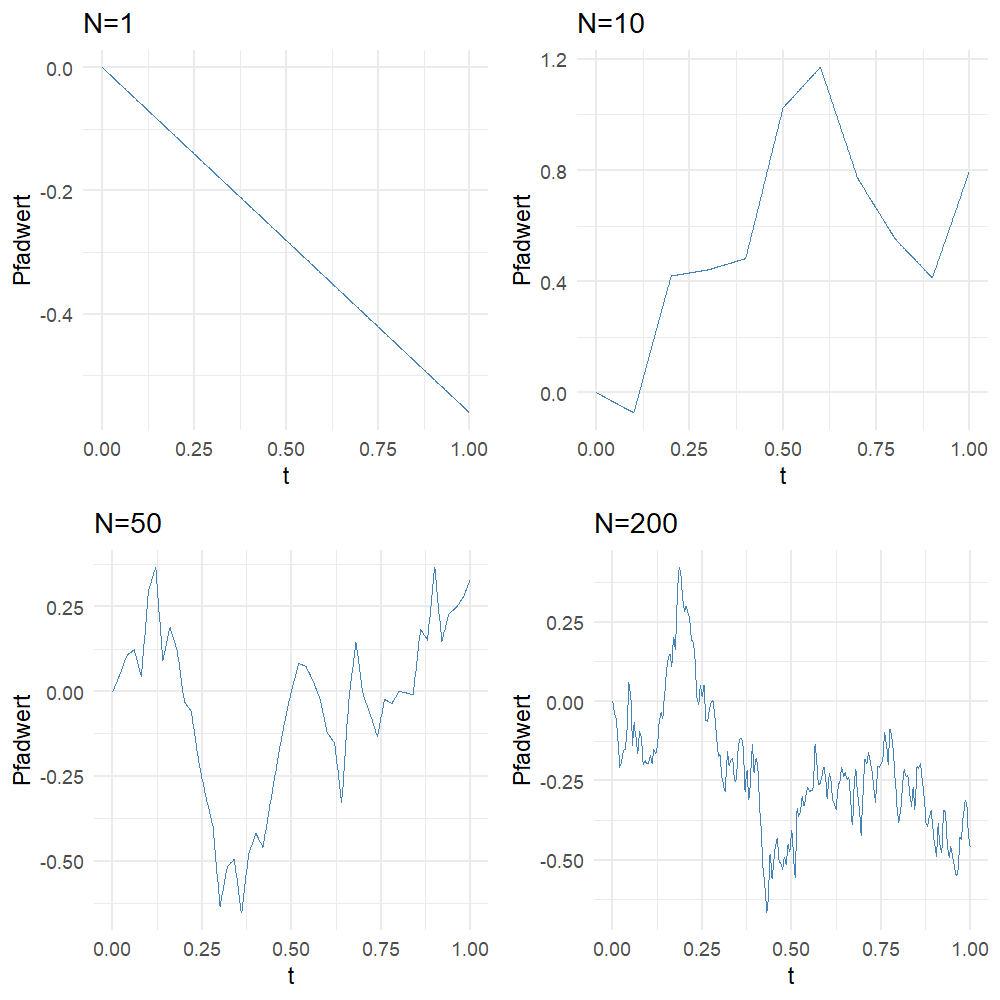
\includegraphics[width=0.9\textwidth]{images/disrete_bb.png}
    \caption{Diskrete Brownsche Bewegung erster, zehnter, fünfzigster und zweihundertster Ordnung}
    \label{fig:brownian}
\end{figure}

\end{bsp}

\begin{lemma}[Martingal-Eigenschaft der diskreten Brownschen Bewegung]
Ohne Beschränkung der Allgemeinheit wird der Fall $N=1$ betrachtet, sonst kann die Zeit skaliert werden.
Ebenso wird nur der Fall $t \in \Bbb N_0$ untersucht: Der Prozess ist also wieder diskret. Das ist
ausreichend, da im Verlauf der Arbeit der Grenzprozess $N \to \infty$ relevant 
wird. Dann ist jeder Wert der Brownschen Bewegung beliebig nah an einem der diskreten Werte, 
und die Martingal-Eigenschaft folgt aus der Stetigkeit des Erwartungswertes. Der stetig interpolierte 
diskrete Prozess an sich ist nämlich kein Martingal. \textit{Beweis.}
Zuerst wird der Fall $m=n+1$ betrachtet: zu zeigen ist
$$E(b^{(1)}(m) | b^{(1)}(n)=v) = v.$$
Da $b^{(1)}(m) = b^{(1)}(n) + \eta_{n+1}$ folgt
$$E(b^{(1)}(m) | b^{(1)}(n)=v) = E(v + \eta_{n+1} | b^{(1)}(n)=v) = v + E(\eta_{n+1}) = v.$$
Nun der allgemeine Fall $m > n+1$: aus dem Satz des iterierten Erwartungswertes folgt
$$E(b^{(1)}(m) | b^{(1)}(n)=v) = E(E(b^{(1)}(m) | b^{(1)}(m-1)) | b^{(1)}(n)=v).$$
Da $E(b^{(1)}(m) | b^{(1)}(m-1)) = b^{(1)}(m-1)$ folgt
$$E(b^{(1)}(m) | b^{(1)}(n)=v) = E(b^{(1)}(m-1) | b^{(1)}(n)=v).$$
Induktiv folgt die Behauptung. \qed \\

\end{lemma}

\begin{lemma}[Varianz der diskreten Brownschen Bewegung]
$$
\begin{aligned}
V(b^{(N)}(t)) &= \frac{1}{N} \left ( V(\xi_{\lfloor Nt \rfloor}) + (Nt - \lfloor Nt \rfloor)^2 \cdot V(\xi_{\lfloor Nt \rfloor + 1} - \xi_{\lfloor Nt \rfloor}) \right ) 
\\ &= \frac{1}{N} (\lfloor Nt \rfloor + (Nt - \lfloor Nt \rfloor)^2)  
\\ &= \frac{\lfloor Nt \rfloor}{N} + \frac{(Nt - \lfloor Nt \rfloor)^2}{N}.
\end{aligned}
$$
Im Grenzübergang $N \to \infty$ konvergiert $\frac{\lfloor Nt \rfloor}{N} \to t$ und $\frac{(Nt - \lfloor Nt \rfloor)^2}{N} \to 0$.
\qed
\end{lemma}

\subsection{Nützliche Ergebnisse aus der Stochastik}
Im Folgenden Beweis zur Stetigkeit der Pfade werden einige Ergebnisse aus der Stochastik verwendet, die hier zusammengefasst, aber nicht bewiesen werden.

\begin{lemma}[Reihenkriterium für fast sichere Konvergenz, Henze \cite{henze} S. 201]
Sei $(X_n)_{n \in \Bbb N}$ eine Folge von Zufallsvariablen. Wenn es eine Reihe $\sum_{n=1}^\infty a_n \lt \infty$ mit $a_n \geq 0$ gibt, so dass
$$P(|X_n| > \varepsilon) \leq a_n \quad \text{für alle } n \in \Bbb N \text{ und jedes } \varepsilon > 0,$$
dann konvergiert $X_n$ fast sicher gegen $0$, d.h.
$$P\left(\lim_{n \to \infty} X_n = 0\right) = 1.$$
Wird hier nicht bewiesen. \qed
\end{lemma}

\begin{satz}[Cramér-Wold-Technik, Henze \cite{henze} S. 225]
Seien $(X_n)_{n \in \Bbb N}$ und $X$ Zufallsvektoren in $\Bbb R^d$. Dann sind folgende Aussagen äquivalent:
\begin{enumerate}
    \item $X_n \xrightarrow{d} X$ für $n \to \infty$.
    \item Für alle $t \in \Bbb R^d$ gilt $t^T X_n \xrightarrow{d} t^T X$ für $n \to \infty$.
\end{enumerate}
Wird hier nicht bewiesen. \qed \\
Die Cramér-Wold-Technik erlaubt es, mehrdimensionale Verteilungskonvergenz auf eindimensionale Berechnungen zurückzuführen.
\end{satz}

\subsection{Die Brownschen Bewegung als Grenzprozess und Eigenschaften}
Nun wird der Grenzprozess $N \to \infty$ betrachtet. Intuitiv wird die Zeit immer feiner aufgelöst,
und es werden immer mehr Normalverteilungen in eine Zeiteinheit einbezogen. Vorerst ist jedoch unklar, 
ob der Grenzprozess überhaupt existiert. Um die Konvergenz des Prozesses zu zeigen, wird die Verteilungskonvergenz 
untersucht. Konvergenz der einzelnen Zeitpunkte (oder endlich-dimensionalen Vektoren) reicht nicht 
für Konvergenz der Prozesse als Funktionen. Dazwischen könten „Spikes“/hochfrequente Oszillationen liegen,
die jede feste endliche Stichprobe verfehlen, aber im Supremumsabstand sichtbar bleiben, zum Beispiel könnte der
Prozess bei irrationalen Zeiten den Wert $\infty$ annehmen (Das ist natürlich nur ein Gedankenexperiment und 
sehr unintuitiv). Daher wird die Konvergenz in 3 Schritten untersucht:
\begin{enumerate}
  \item Verteilungskonvergenz der einzelnen Zeitpunkte
  \item Verteilungskonvergenz von endlich-dimensionalen Vektoren und die Kovarianzen
  \item Stetigkeit der Pfade des Grenzprozesses
\end{enumerate}

\begin{lemma}[Verteilungskonvergenz der diskreten Brownschen Bewegung]
Es existiert ein stochastischer Prozess $W_t, t \geq 0$, so dass für jedes $t$ die Verteilung von $b^{(N)}(t)$ gegen die Verteilung von $W_t$ konvergiert, wenn $N \to \infty$.
\textit{Beweis.}
Da 
$$b^{(N)}(t) = \frac{1}{\sqrt{N}}\big(\xi_k+\alpha(\xi_{k+1}-\xi_k)\big)
=\frac{1}{\sqrt{N}}\big(\xi_k+\alpha\,\eta_{k+1}\big).
$$
ist $b^{(N)}(t)$ eine lineare Kombination von Normalverteilungen, und daher widerum 
normalverteilt. Erwartungswert und Varianz wurden bereits berechnet:
$$
E(b^{(N)}(t)) = 0, \quad V(b^{(N)}(t)) = \sigma_N^2(t) = \frac{1}{N}\big(k+\alpha^2\big),
$$
wobei $k=\lfloor Nt \rfloor$ und $\alpha=Nt-k\in[0,1)$. Damit gilt
$$
b^{(N)}(t) \sim N\left(0,\frac{1}{N}\big(k+\alpha^2\big)\right).
$$
Die Verteilungsfunktion ist gegeben durch
$$
F_N(x)=P\big(b^{(N)}(t)\le x\big)=\Phi\!\left(\frac{x}{\sigma_N(t)}\right),
$$
wobei $\Phi$ die Standardnormalverteilungsfunktion ist. Aus $\sigma_N^2(t)\to t$ folgt $\sigma_N(t)\to \sqrt{t}$ und wegen der Stetigkeit von $\Phi$ daher
$$
F_N(x)=\Phi\!\left(\frac{x}{\sigma_N(t)}\right)\;\longrightarrow\;\Phi\!\left(\frac{x}{\sqrt{t}}\right)\quad\text{für alle }x\in\Bbb R.
$$
Dies ist die Verteilungsfunktion von $N(0,t)$. Definiere $W_t :\sim N(0,t)$. Somit konvergiert für jedes feste $t$ die Verteilung von $b^{(N)}(t)$ gegen die von $W_t$. 
\qed
\end{lemma}

\begin{satz}[Kovarianzstruktur der Brownschen Bewegung]
Aus der Verteilungskonvergenz der einzelnen Zeitpunkte kann man noch keinen sinnvollen Grenzprozess folgern.
Die Zeitpunkte $W_t$ sind zwar normalverteilt, aber der Prozess könnte trotzdem sprunghaft sein.
Nun wird die Verteilungskonvergenz der endlich-dimensionalen Vektoren gezeigt, beziehungsweise
die Kovarianz der Realisierungen bei benachbarten Zeitpunkten untersucht.
Sei $0\le t_1\le\cdots\le t_k$ eine Zerlegung. Dann gilt
$$
\big(b^{(N)}(t_1), \dots , b^{(N)}(t_k) \big )\;\xrightarrow[N \to \infty]{\mathrm{d}}\;\big(W_{t_1},\dots,W_{t_k}\big).
$$
\textit{Beweis.}\footnote{angelehnt an Henze \cite{henze} S. 225f.}
Für jedes $N$ ist der Vektor $\big(b^{(N)}(t_1),\dots,b^{(N)}(t_k)\big)$ gemeinsam normalverteilt,
denn $b^{(N)}(t)$ ist eine lineare Kombination der i.i.d. Standardnormalen $(\eta_i)$.

Es genügt, Mittelwerte und Kovarianzen zu kontrollieren:
Die Mittelwerte sind Null. Für $s,t\ge0$ mit $k=\lfloor Nt\rfloor$, $\alpha=Nt-k$, 
$\ell=\lfloor Ns\rfloor$, $\beta=Ns-\ell$ gilt mit $\xi_n=\sum_{i=1}^n\eta_i$:
$$
b^{(N)}(t)=\tfrac1{\sqrt N}\big(\xi_k+\alpha\eta_{k+1}\big),\qquad
b^{(N)}(s)=\tfrac1{\sqrt N}\big(\xi_\ell+\beta\eta_{\ell+1}\big).
$$
Unabhängigkeit der $\eta_i$ liefert
$$
\mathrm{Cov}\!\big(b^{(N)}(s),b^{(N)}(t)\big)
=\frac1N\Big(\min(\ell,k)+\alpha\,\mathbf 1_{\{k+1\le \ell\}}+\beta\,\mathbf 1_{\{\ell+1\le k\}}+\alpha\beta\,\mathbf 1_{\{\ell=k\}}\Big).
$$
Damit
$$
\mathrm{Cov}\!\big(b^{(N)}(s),b^{(N)}(t)\big)
=\frac{\min(\ell,k)}{N}+O\!\left(\frac1N\right)\xrightarrow[N\to\infty]{}\min(s,t).
$$
Folglich konvergiert die Kovarianzmatrix der Vektoren gegen 
$\Sigma=(\min(t_i,t_j))_{i,j}$.
Nach der Cramér–Wold-Technik reicht es, lineare Formen zu betrachten. Sei also $a=(a_1,\dots,a_k)^\top\in\Bbb R^k$ und
$$
Y_N:=\sum_{i=1}^k a_i\,b^{(N)}(t_i),\qquad
Y:=\sum_{i=1}^k a_i\,W_{t_i}.
$$
Für jedes $N$ ist $Y_N$ zentriert normalverteilt und
$$
\mathrm{Var}(Y_N)=\sum_{i,j=1}^k a_i a_j\,\mathrm{Cov}\!\big(b^{(N)}(t_i),b^{(N)}(t_j)\big).
$$
Mit der oben gezeigten Kovarianzkonvergenz folgt
$$
\mathrm{Var}(Y_N)\xrightarrow[N\to\infty]{}\sum_{i,j=1}^k a_i a_j\,\min(t_i,t_j)=:\sigma^2(a).
$$
Damit gilt wegen der Eindeutigkeit zentrierter Normalverteilungen durch ihre Varianz
$$
Y_N \xrightarrow[N\to\infty]{} N\!\big(0,\sigma^2(a)\big).
$$
Zugleich ist $Y$ normalverteilt mit
$$
\mathrm{Var}(Y)=\sum_{i,j=1}^k a_i a_j\,\mathrm{Cov}(W_{t_i},W_{t_j})
=\sum_{i,j=1}^k a_i a_j\,\min(t_i,t_j)=\sigma^2(a).
$$
Also konvergiert für jedes $a$ die Verteilung von $a^\top(b^{(N)}(t_1),\dots,b^{(N)}(t_k))$ gegen die von $a^\top(W_{t_1},\dots,W_{t_k})$.
Nach Cramér–Wold folgt die behauptete Verteilungskonvergenz des Vektors. \qed
\end{satz}



\begin{bem}[Sinn und Zweck des letzten Satzes]
Um die Wichtigkeit der Kovarianz-Struktur zu verdeutlichen, wird in der folgenden Visualisierung gezeigt, wie ein
stochastischer Prozess ohne Kovarianz der einzelnen Zufallsvariablen aussehen würde.
In Blau werden die Verteilungen der Zufallsvariablen, und in Rot jeweils Realisierungen des Prozesses dargestellt.
In der zweiten Grafik (mit Kovarianz-Struktur) kann man beobachten, das die Verteilungen eine geringere Varianz haben, und jeweils um den Vorherigen Wert zentriert sind. Dies wird im Folgenden noch präzisiert.
Das kann man als ein Stetigkeits-Kriterium betrachten. (Obwohl man nicht direkt auf die Stetigkeit der Pfade folgern kann)

Ausgehend von der Kovarianz-Struktur kann man die Stetigkeit mit dem Stetigkeitssatz von Kolmogorov (Behrends \cite{behrends}, 2013, S. 78f.) folgern.
In dieser Arbeit wird jedoch ein anderer Beweisansatz genutzt.

\begin{figure}[H]
    \centering
    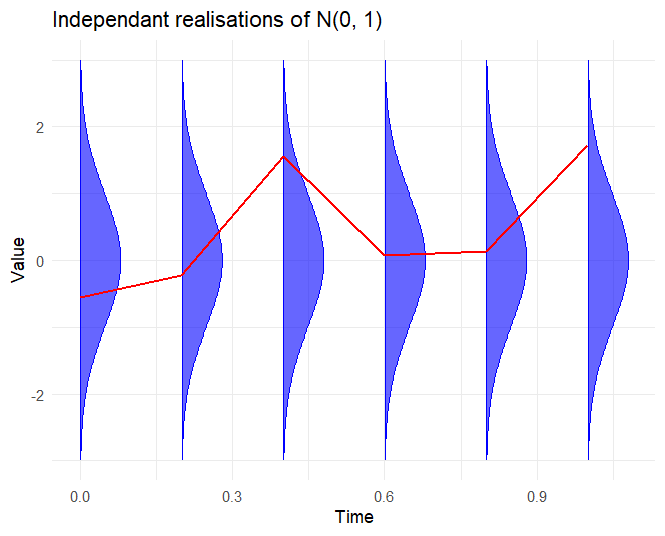
\includegraphics[width=\textwidth]{images/bb_without_cov.png}
    \caption{Folge von Normalverteilten Zufallsvariablen ohne Kovarianz}
    \label{fig:bb_without_cov}

    \centering
    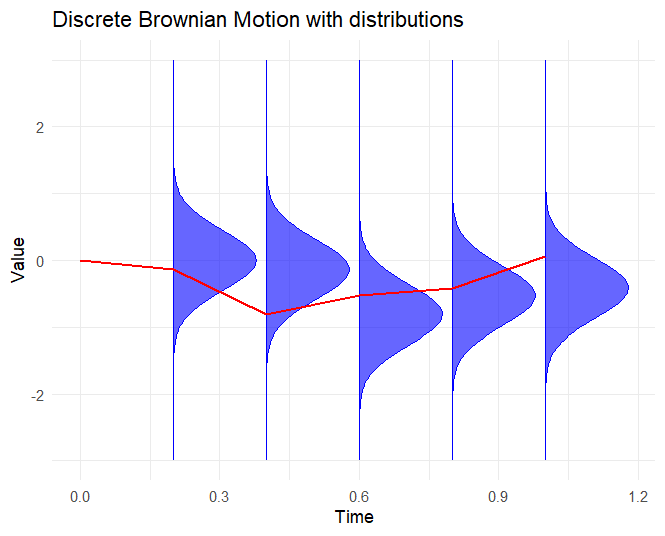
\includegraphics[width=\textwidth]{images/bb_with_cov.png}
    \caption{Visualierung der Verteilung der diskreten Brownschen Bewegung unter Beachtung der Kovarianzstruktur}
    \label{fig:bb_with_cov}

\end{figure}
\end{bem}

\begin{satz}[Selbstähnlichkeit und bedingte Verteilung der Brownschen Bewegung]
Für jedes $c > 0$ gilt
$$
W_{ct}(\omega) \overset{d}{=} \sqrt{c}\, W_t(\omega) \quad \text{für alle } t \ge 0,
$$
für alle $s < t$ gilt
$$
W_t - W_s \sim N(0, t-s),
$$
und die bedingte Verteilung von $W_t$ gegeben $W_s$ ist
$$
W_t \mid W_s \sim N\big(W_s, t-s\big).
$$
\textit{Beweis der ersten Behauptung (Selbstähnlichkeit).} \\
Für $t \ge 0$ gilt $W_{ct} \sim N(0, ct)$ und $W_t \sim N(0, t)$. Somit gilt
$$
\sqrt{c}\, W_t \sim N(0, c t).
$$
Da beide Normalverteilungen denselben Mittelwert $0$ und dieselbe Varianz $ct$ haben, folgt
$$
W_{ct} \stackrel{d}{=} \sqrt{c}\, W_t \quad \text{für jedes } t \ge 0.
$$  
\qed  \\
\textit{Beweis der zweiten Behauptung (Inkremente).} \\
Für $s < t$ gilt
$$
W_t - W_s = \lim_{N \to \infty} \big( b^{(N)}(t) - b^{(N)}(s) \big),
$$
wobei $b^{(N)}$ diskrete Approximierungen sind. Jedes Inkrement $b^{(N)}(t) - b^{(N)}(s)$ ist normalverteilt mit Erwartungswert $0$ und Varianz $t-s$. Durch Grenzwertbildung folgt
$$
W_t - W_s \sim N(0, t-s).
$$
\qed  \\
\textit{Beweis der dritten Behauptung (Bedingte Verteilung).} \\
Betrachte $(W_s, W_t)^T$, das multivariat normal verteilt ist mit
$$
E(W_s) = E(W_t) = 0, \quad
\mathrm{Cov}(W_s, W_t) = \min(s, t) = s.
$$  
Die Kovarianzmatrix lautet somit
$$
\Sigma = \begin{pmatrix} s & s \\ s & t \end{pmatrix}.
$$
Für die bedingte Verteilung ergibt die Standardformel der multivariaten Normalverteilung
$$
\begin{aligned}
E(W_t \mid W_s) &= E(W_t) + \mathrm{Cov}(W_t, W_s)\,V(W_s)^{-1} (W_s - E(W_s)) \\
&= 0 + \frac{s}{s} W_s = W_s, \\
V(W_t \mid W_s) &= V(W_t) - \frac{\mathrm{Cov}(W_t, W_s)^2}{V(W_s)} \\
&= t - \frac{s^2}{s} = t - s.
\end{aligned}
$$
Insgesamt folgt
$$
W_t \mid W_s \sim N(W_s,\, t-s).
$$ \qed
\end{satz}

\begin{korr}[Martingal-Eigenschaft der Brownschen Bewegung]
Die Brownsche Bewegung $W_t$ ist ein Martingal.
\textit{Beweis.} Aus dem vorigen Satz folgt
$$
E(W_t | W_s = v) = v.
$$
Damit ist $W_t$ ein Martingal. \qed
\end{korr}  

\begin{satz}[Stetigkeit der Pfade]
Der Pfad $t \mapsto W_t(\omega)$ ist fast sicher stetig.
\textit{Beweis.}
Für den Beweis wird eine neue Funktionen-Folge $\hat W_t^{(n)}(\omega), n \in \Bbb N$
definiert, wobei $\hat W_t^{(n)}(\omega)$ die lineare Interpolation der Werte $W_{k/2^n}(\omega), k=0,1,2,\ldots$ ist. 
Ohne Beschränkung der Allgemeinheit wird das Intervall $[0,1]$ betrachtet. Für $n \in \Bbb N$ und $k=0,\dots,2^n-1$ setze
$$I_{n,k}:=\big[k2^{-n},(k+1)2^{-n}\big].$$
Da die $I_{n,k}$ eine Zerlegung von $[0,1]$ bilden, ist
$$
\begin{aligned}
M_n &:=\sup_{t\in[0,1]}\big|\hat W^{(n+1)}_t-\hat W^{(n)}_t\big| 
\\ &= \max_{0\le k<2^n} \sup_{t\in I_{n,k}} \big|\hat W^{(n+1)}_t-\hat W^{(n)}_t\big| =\max_{0\le k<2^n}|Z_{n,k}|
\end{aligned}
$$
Für die unabhängigen Inkremente $Z_{n,k}$ mit
$$
Z_{n,k}\sim N\!\big(0,2^{-(n+2)}\big).
$$
Für eine Normalverteilung $Z\sim N(0,\sigma^2)$ und jedes $\varepsilon>0$ gilt (siehe z. B. Boucheron 2013 \cite{boucheron_concentration_2013} S. 2)
$$
P(|Z|>\varepsilon) \le 2\exp\!\Big(-\frac{\varepsilon^2}{2\sigma^2}\Big).
$$
Mit der Vereinigungsschranke folgt damit
$$
P(M_n>\varepsilon) \le \sum_{k=0}^{2^n-1} P(|Z_{n,k}|>\varepsilon)
\le 2^n\cdot 2\exp\!\Big(-\frac{\varepsilon^2}{2\sigma_n^2}\Big)
= 2^{\,n+1}\exp\!\Big(-\frac{\varepsilon^2}{2\sigma_n^2}\Big).
$$
Man wählt nun eine spezifische Folge $\varepsilon_n$ so, dass sich aus der rechten Seite eine geometrische Reihe ergibt. Setze
$$
\varepsilon_n := \sqrt{2(n+1)}\,\sigma_n.
$$
Dann gilt
$$
\frac{\varepsilon_n^2}{2\sigma_n^2}=n+1,
$$
und damit
$$
P(M_n>\varepsilon_n)\le 2^{\,n+1} e^{-(n+1)} = \big(2e^{-1}\big)^{\,n+1}.
$$
Da $2e^{-1}<1$ ist, ist die Folge auf der rechten Seite geometrisch und insbesondere summierbar. Folglich
$$
\sum_{n=1}^\infty P(M_n>\varepsilon_n) < \infty.
$$
Nach dem Reihenkriterium für fast sichere Konvergenz folgt, dass $M_n\to 0$ fast sicher.
Für $m \gt n \ge N$ beliebig gilt
$$\sup_{t}|\hat W^{(m)}_t - \hat W^{(n)}_t| \leq \sum_{k=n}^{m-1} M_k. \underset{N \to \infty} \longrightarrow 0$$
Weil jedes $\big(\hat W^{(n)}\big)_{n\in\Bbb N}$ eine stückweise lineare Funktion ist, folgt
dass $\big(\hat W^{(n)}\big)_{n\in\Bbb N}$ fast sicher eine Cauchy-Folge in $\Vert \cdot \Vert_{\infty}$ ist.
$\big(\hat W^{(n)}\big)_{n\in\Bbb N}$ konvergiert also gleichmäßig gegen den Grenzpfad $\widetilde W$, der stetig ist. \qed

Achtung: Es wurde nicht gezeigt, der Prozess $W_t^{(n)} \longrightarrow W_t$ gleichmäßig konvergiert. Für eine beliebige aber feste Realisierung
$t \mapsto W_t(\omega)$ wurde eine (reellwertige) Folge von stetigen Funktionen konstruiert, die gegen $t \mapsto W_t$ gleichmäßig konvergiert.
Da es sich um eine Folge stetiger Funktionen handelt, gilt die Stetigkeit unter gleichmäßiger Konvergenz auch gegen die Grenzfunktion $t \mapsto W_t$.
\end{satz}

\section{Die geometrische Brownsche Bewegung}

Die geometrische Brownsche Bewegung ist eine Erweiterung der Brownschen Bewegung. 
Sie eignet zur Modellierung von Aktienkursen, da sie im Gegensatz zur klassischen 
Brownschen Bewegung stets positive Werte annimmt.


\subsection{Die geometrische Brownschen Bewegung}

Das \textit{Binomialmodell} beschreibt den Aktienkurs $S_t$ in diskreter Zeit: In jedem Zeitschritt ändert sich der Kurs multiplikativ um einen Zufallsfaktor. Es gilt
$$
S_{k+1} = S_k \,(1 + X_{k+1}), \qquad k = 0,1,\dots,n-1,
$$
für eine Zufallsvariable $X_{k+1}$ die die relative Kursänderung im Schritt $k+1$ repräsentiert. Um eine kontinuierliche Zeitentwicklung zu modellieren, 
setzt man\footnote{Dies ist ein Schritt des Euler-Verfahren zur numerischen Lösung der 
stochastischen Differentialgleichung der geometrischen Brownschen Bewegung. \cite{iacus2008}, S. 68.}
$$
X_{k+1} = \mu  \Delta t + \sigma \sqrt{\Delta t}\varepsilon_{k+1},
$$
mit $\mu$ als Erwartungswert der Rendite (oder auch Drift), $\sigma$ als Volatilität, und $\varepsilon_{k+1}$ unabhängig, identisch verteilten Zufallsvariablen mit Erwartungswert $0$ und Varianz $1$. 
(An dieser Stelle ist unwichtig, wie die $\varepsilon_{k+1}$ verteilt sind, es reicht, dass sie diese Momente besitzen. 
Die Information über die Verteilung wird in einem Grenzübergang verloren gehen.)
Das bildet die Modellannahme für den Rest dieser Arbeit.

Im Folgenden wird eine explizite Formel für $S_t$ bewiesen, nämlich
$$S_T = S_0 \exp\!\Big( (\mu - \tfrac12 \sigma^2)T + \sigma W_T \Big),$$
wobei $W_T$ eine Brownsche Bewegung ist und $T=n \cdot \Delta t$. \textit{Beweis.}
Man betrachtet den Logarithmus der $S_k$: Nach $n$ Schritten ist der Aktienkurs
$$
S_n = S_0 \prod_{j=1}^n (1 + X_j).
$$
Durch den Logarithmus erhält man
\begin{equation} \label{eq:log_sn}
\log S_n = \log S_0 + \sum_{j=1}^n \log(1+X_j).
\end{equation}
Als nächstes wird die Taylor-Entwicklung der Terme $\log(1+X_j)$ betrachtet. Die $k$-te Ableitung lautet
$$\log(1+x)^{(k)}=(-1)^{k+1} \frac{(k-1)!}{(1+x)^k}.$$
Setzt man diese in die Taylor-Formel ein ergibt sich
$$\log(1+x) = \sum_{k=0}^{\infty} \frac{(\log(1+\cdot)^{(k)})(0)}{k!}(x-0)^k= \sum_{k=1}^\infty(-1)^{k+1} \frac{x^k}{k}$$
Da $X_j \in O(\sqrt{\Delta t})$ ist, reicht die Taylor-Entwicklung bis zum quadratischen Term: Es gilt
$$
X_j^k = (\mu \Delta t + \sigma \sqrt{\Delta t} \varepsilon_j)^k.
$$
Durch den Binomischen Lehrsatz ergibt sich:
$$
X_j^k = \sum_{m=0}^k \binom{k}{m} (\mu \Delta t)^{k-m} (\sigma \sqrt{\Delta t} \varepsilon_j)^m.
$$
Die Terme enthalten Potenzen von $\Delta t$ in der Form $(\Delta t)^{(k-m) + m/2} = (\Delta t)^{k-m/2}$. Für $k \geq 3$ (und $m=0,\dots k$) ist $(\Delta t)^{k-m/2}$ von 
höherer Ordnung als $\Delta t$ oder $\sqrt{\Delta t}$ und verschwindet daher im Grenzübergang $\Delta t \to 0$ bzw. $n \to \infty$. Der Grenzübergang 
von diskreter zu kontinuierlicher Zeit führt eben dazu, dass $n$ und $\Delta t$ gleichzeitig gegen $\infty$ bzw. $0$ gehen, wobei $n \Delta t = T$ konstant bleibt.
Daher verschwinden in der Summe in Formel \ref{eq:log_sn} genau die Terme, in denen $\Delta t$ einen Exponenten größer $1$ hat.
$$
\log(1+X_j) \approx X_j - \tfrac12 X_j^2.
$$
Der quadratische Term wird nun ausmultipliziert und in der selben Weise abgeschätzt:
$$
\tfrac12 X_j^2 \approx \tfrac12 \sigma^2 \Delta t \,\varepsilon_j^2.
$$
Hier verschwinden die Terme $\mu (\Delta t)^2 \in o((\Delta t)^{2})$ und $2 \mu (\Delta t) \sigma \sqrt{\Delta t} \varepsilon_{k+1} \in o((\Delta t)^{3/2})$ wieder im Limes. Zwischenfazit:
$$
\begin{aligned}
\log S_n &\approx \log S_0 + \sum_{j=1}^n\left( \underbrace{\mu \Delta t + \sigma\sqrt{\Delta t} \varepsilon_j}_{X_j} - \underbrace{\frac{1}{2} \sigma^2 \Delta t \varepsilon_j}_{-\frac{1}{2} X_j^2} \right)
\\ &= \log S_0 + \mu T + \sigma\sqrt{\Delta t} \sum_{j=1}^{n} \varepsilon_j - \frac{1}{2} \sigma^2 \sum_{j=1}^{n} \Delta t \varepsilon_j^2 
\end{aligned}
$$
Im Folgenden wird der Grenzübergang $n \longrightarrow \infty$ bzw. $\Delta t \longrightarrow 0$ durchgeführt. 
Die erste Summe konvergiert nach dem Zentralen Grenzwertsatz (Verteilungskonvergenz):
$$
\sigma \sqrt{\Delta t} \sum_{j=1}^n \varepsilon_j = \sigma \frac{\sqrt{T}}{\sqrt{N}} \sum_{j=1}^n \varepsilon_j  \xrightarrow[n \to \infty]{\mathrm{d}} \xi \sim \mathcal N(0, \sigma^2 T),
$$
also gegen eine Zufallsvariable $\xi$ die normalverteilt ist, mit Varianz $\sigma^2 T$.  $\xi = \sigma W_T$ ist eine Lösung, 
weil $W_T \sim \mathcal N(0, T)$ eine Brownsche Bewegung zur Zeit $T$ ist. 
Da $E(\varepsilon_j)=0$ und $V(\varepsilon_j)=1$ und damit $E(\varepsilon_j^2) = 1$ gilt, folgt im Grenzübergang für die zweite Summe nach dem Gesetz der großen Zahlen
$$
\frac{1}{2} \sigma^2 \sum_{j=1}^{n} \Delta t \varepsilon_j^2  \xrightarrow[n \to \infty]{\mathrm{f.s.}} \tfrac12 \sigma^2 T.
$$
Damit ergibt sich im Grenzübergang $n \to \infty$:
$$
\log S_T \overset{d} = \log S_0 + \big(\mu - \tfrac12 \sigma^2\big)T + \sigma W_T.
$$Exponentiell geschrieben erhält man die \textit{geometrische Brownsche Bewegung}:
$$
S_T \overset d = S_0 \exp\!\Big( (\mu - \tfrac12 \sigma^2)T + \sigma W_T \Big).
$$
\qed
\subsection{Die logarithmische Normalverteilung}

Eine Zufallsvariable $X$ heißt log-Normalverteilt mit Varianz $\sigma^2$ und Erwartungswert $\mu$, 
falls die Zufallsvariable $Y := \log(X)$ normalverteilt ist mit $Y \sim \mathcal N(\mu, \sigma^2)$.
$S_T$ ist somit log-normalverteilt:
$$\log S_T \overset{d} = \log S_0 + \big(\mu - \tfrac12 \sigma^2\big)T + \sigma W_T.$$
ergibt
$$\log S_T \sim N\left( \log S_0 + \left( \mu - \frac{1}{2} \sigma^2 \right)T , \sigma^2 T\right)$$
Erwartungswert und Varianz eines Kurses zum Zeitpunkt $T$ sind damit
$$E(S_T)=\log S_0 + (\mu - \tfrac12 \sigma^2)T, \quad V(S_T)=\sigma^2 T.$$


\section{Anwendungen auf Zeitreihen}

\subsection{Kalibrierung}
Aus einem Datensatz lassen sich die Parameter $\mu$ und $\sigma$ der
geometrischen Brownschen Bewegung schätzen. 
Für reale Werte ist $\Delta t \gt 0$ und $n$ ist die (endliche) Anzahl von Datenpunkten. 
Zur Schätzung von $\mu$ und $\sigma$ werden die log-Rendite
$$r_j := \log S_j - \log S_{j-1}= \big(\mu - \tfrac12 \sigma^2\big)\Delta t + \sigma (W_j - W_{j-1})$$
genutzt. Da $W_j - W_{j-1} \sim N(0, \Delta t)$ folgt
$$r_j \sim N((\mu - \tfrac12 \sigma^2)\Delta t, \sqrt{\sigma} \Delta t).$$
Man berechnet also die log-Rendite $\hat r_j$ des Datensatzes, 
und davon den empirischen Erwartungswert $m$ (den Durchschnitt) und die empirische Varianz $s^2$. 
Dann folgt $$\sigma \approx s,\quad \mu \approx m + \frac{1}{2} s^2.$$
Die Schätzung der Parameter kann in R wie folgt durchgeführt werden:

\begin{lstlisting}
log_returns <- diff(log(dax$Price)) # tägliche Werte
sigma <- sd(log_returns)
mu <- mean(log_returns) + 0.5 * sigma^2
\end{lstlisting}

\subsection{Back-Tests}

\begin{lemma}[Metriken für Zeitreihenschätzungen]
\end{lemma}


\subsection{Bootstrap-Verfahren zur Kalibrierung}

\subsection{Berechnung von Konfidenzintervallen}

Da $S_T$ log-normalverteilt ist, reicht es ein Konfidenzintervall für die log-Normalverteilung
zu berechnen.
Sei $X \sim N(\mu, \sigma^2)$ eine normalverteilte Zufallsvariable.
Dann ist $Y := e^X$ log-normalverteilt mit Parametern $\mu$ und $\sigma^2$.
Ein zweiseitiges Konfidenzintervall für $X$ mit Konfidenzniveau $1-\alpha$ ist
$$[\mu - z_{\alpha/2} \sigma, \mu + z_{\alpha/2} \sigma],$$
wobei $z_{\alpha/2}$ das $(1-\alpha/2)$-Quantil der Standardnormalverteilung ist.
Exponentiell transformiert ergibt sich das Konfidenzintervall für $Y$:
$$[e^{\mu - z_{\alpha/2} \sigma}, e^{\mu + z_{\alpha/2} \sigma}].$$

\begin{bsp}[Konfidenzintervall für den DAX]

Im folgenden R-Programm (Ausschnitt) wird ein 95\%-Konfidenzintervall für den DAX in einem Jahr von heute (252 Handelstage) berechnet.
Dazu werden die Parameter $\mu$ und $\sigma$ wie oben aus den täglichen log-Renditen geschätzt.

\begin{lstlisting}
alpha = 0.05
T <- 252
z <- qnorm(c(1 - alpha/2, alpha/2))
ci <- S0 * exp((mu - 0.5 * sigma^2) * T + z * sigma * sqrt(T))
\end{lstlisting}

Hier ist $S_0$ der heutige Kurswert des DAX. Das Konfidenzintervall lautet in diesem Fall:
$$[17217, 40097].$$

\end{bsp}

\begin{bsp}[Konfidenzband für den DAX]

Im folgenden R-Programm (Ausschnitt) wird ein 95\%-Konfidenzband für den DAX im naechsten Jahr (252 Handelstage) berechnet.

\begin{lstlisting}
alpha = 0.05
n <- 252
last_date <- max(dax$Date)
future_dates <- last_date + 1:n

q_low <- S0 * exp((mu - 0.5 * sigma^2) * (1:n) + qnorm(1 - alpha/2) * sigma * sqrt((1:n)))
q_hi  <- S0 * exp((mu - 0.5 * sigma^2) * (1:n) + qnorm(alpha/2) * sigma * sqrt((1:n)))
q_med <- S0 * exp((mu - 0.5 * sigma^2) * (1:n))

band <- data.frame(Date = future_dates, low = q_low, mid = q_med, hi = q_hi)
\end{lstlisting}

Es folgt eine Visualisierung des Konfidenzbandes im Anschluss an die historischen Daten.

\begin{figure}[H]
    \centering
    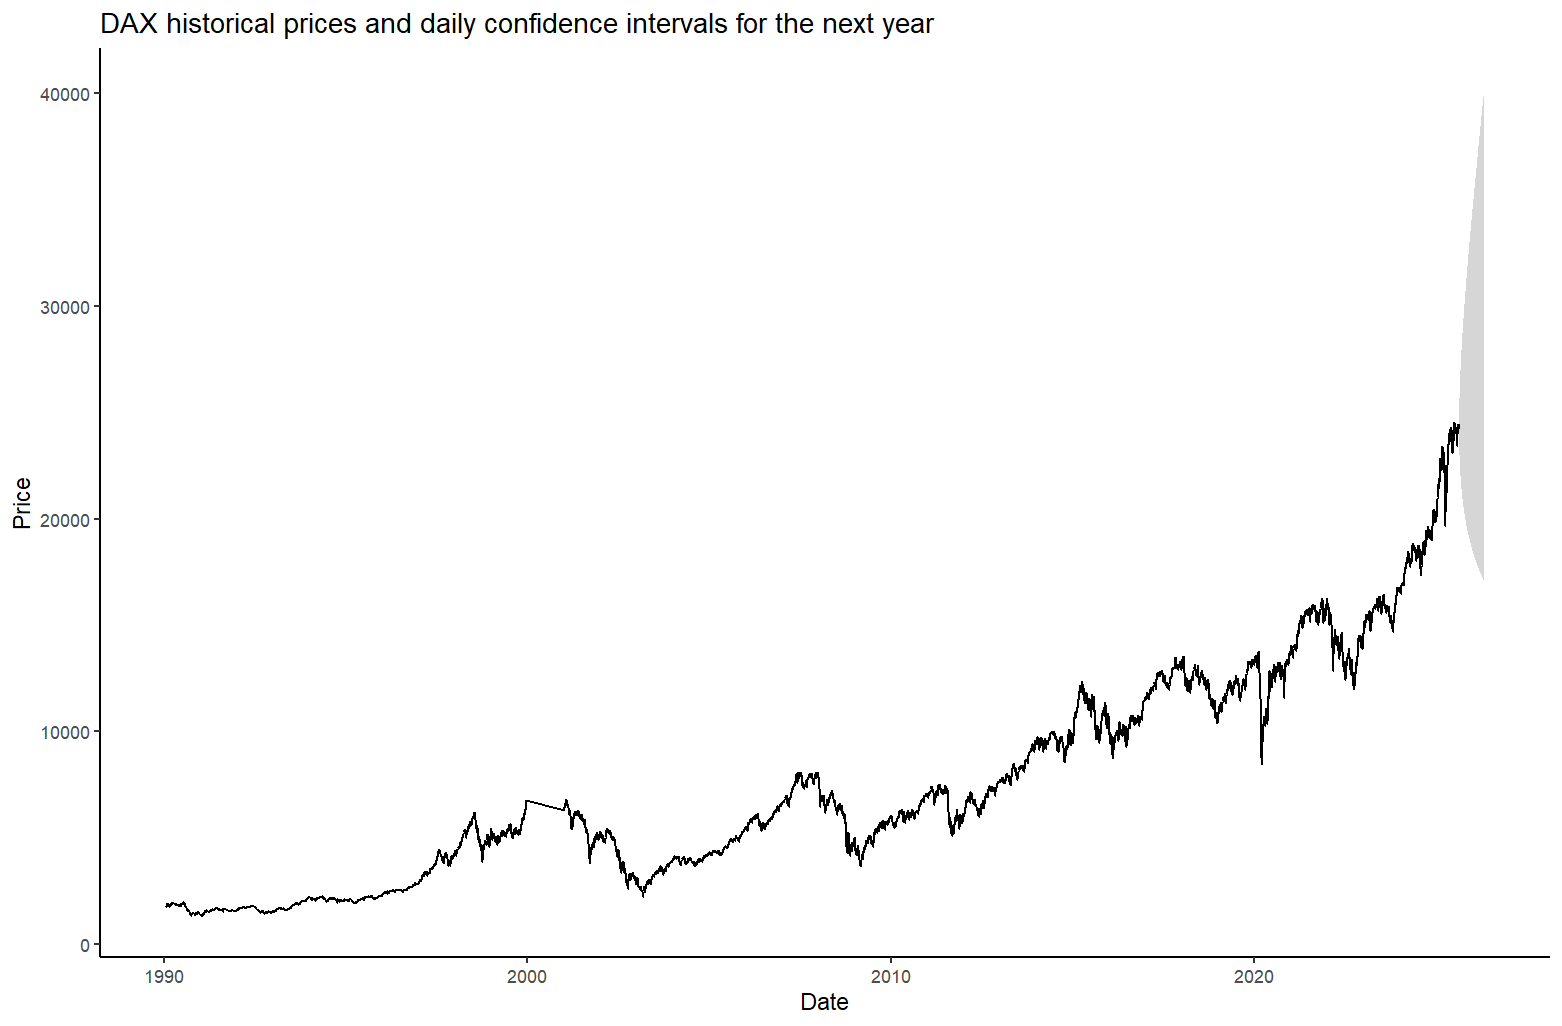
\includegraphics[width=0.9\textwidth]{images/dax_confidence_band.png}
    \caption{DAX mit 95\%-Konfidenzband für das nächste Jahr}
    \label{fig:dax_confidence_band}
\end{figure}

\end{bsp}

\subsection{Monte-Carlo-Simulation}

Genauso wie man eine Brownsche Bewegung mit summierten Normalverteilungen simuliert, 
wird eine geometrische Brownsche Bewegung durch exponentiell transformierte
summierte Normalverteilungen simuliert. 


\begin{bsp}[Monte-Carlo-Simulation des DAX]
Theoretisch liegt das stetige Modell zugrunde, 
aber in der Praxis wird eine diskrete Approximation verwendet, hier mit täglichen Schritten.
Der folgende R-Code (Ausschnitt) simuliert 1000 Pfade der geometrischen Brownschen Bewegung
mit den oben geschätzten Parametern $\mu$ und $\sigma$ für den DAX, wieder für das nächste Jahr (252 Handelstage).

\begin{lstlisting}
n <- 252
paths <- 10000
S0 <- tail(dax$Price, 1)

simulations <- replicate(paths, {
  W <- c(0, cumsum(rnorm(n, 0, 1)))
  S0 * exp((mu - 0.5 * sigma^2) *  c(0, (1:n)) + sigma * W)
})
\end{lstlisting}
Es folgt eine Visualisierung der Simulation im Anschluss an die historischen Daten.

\begin{figure}[H]
    \centering
    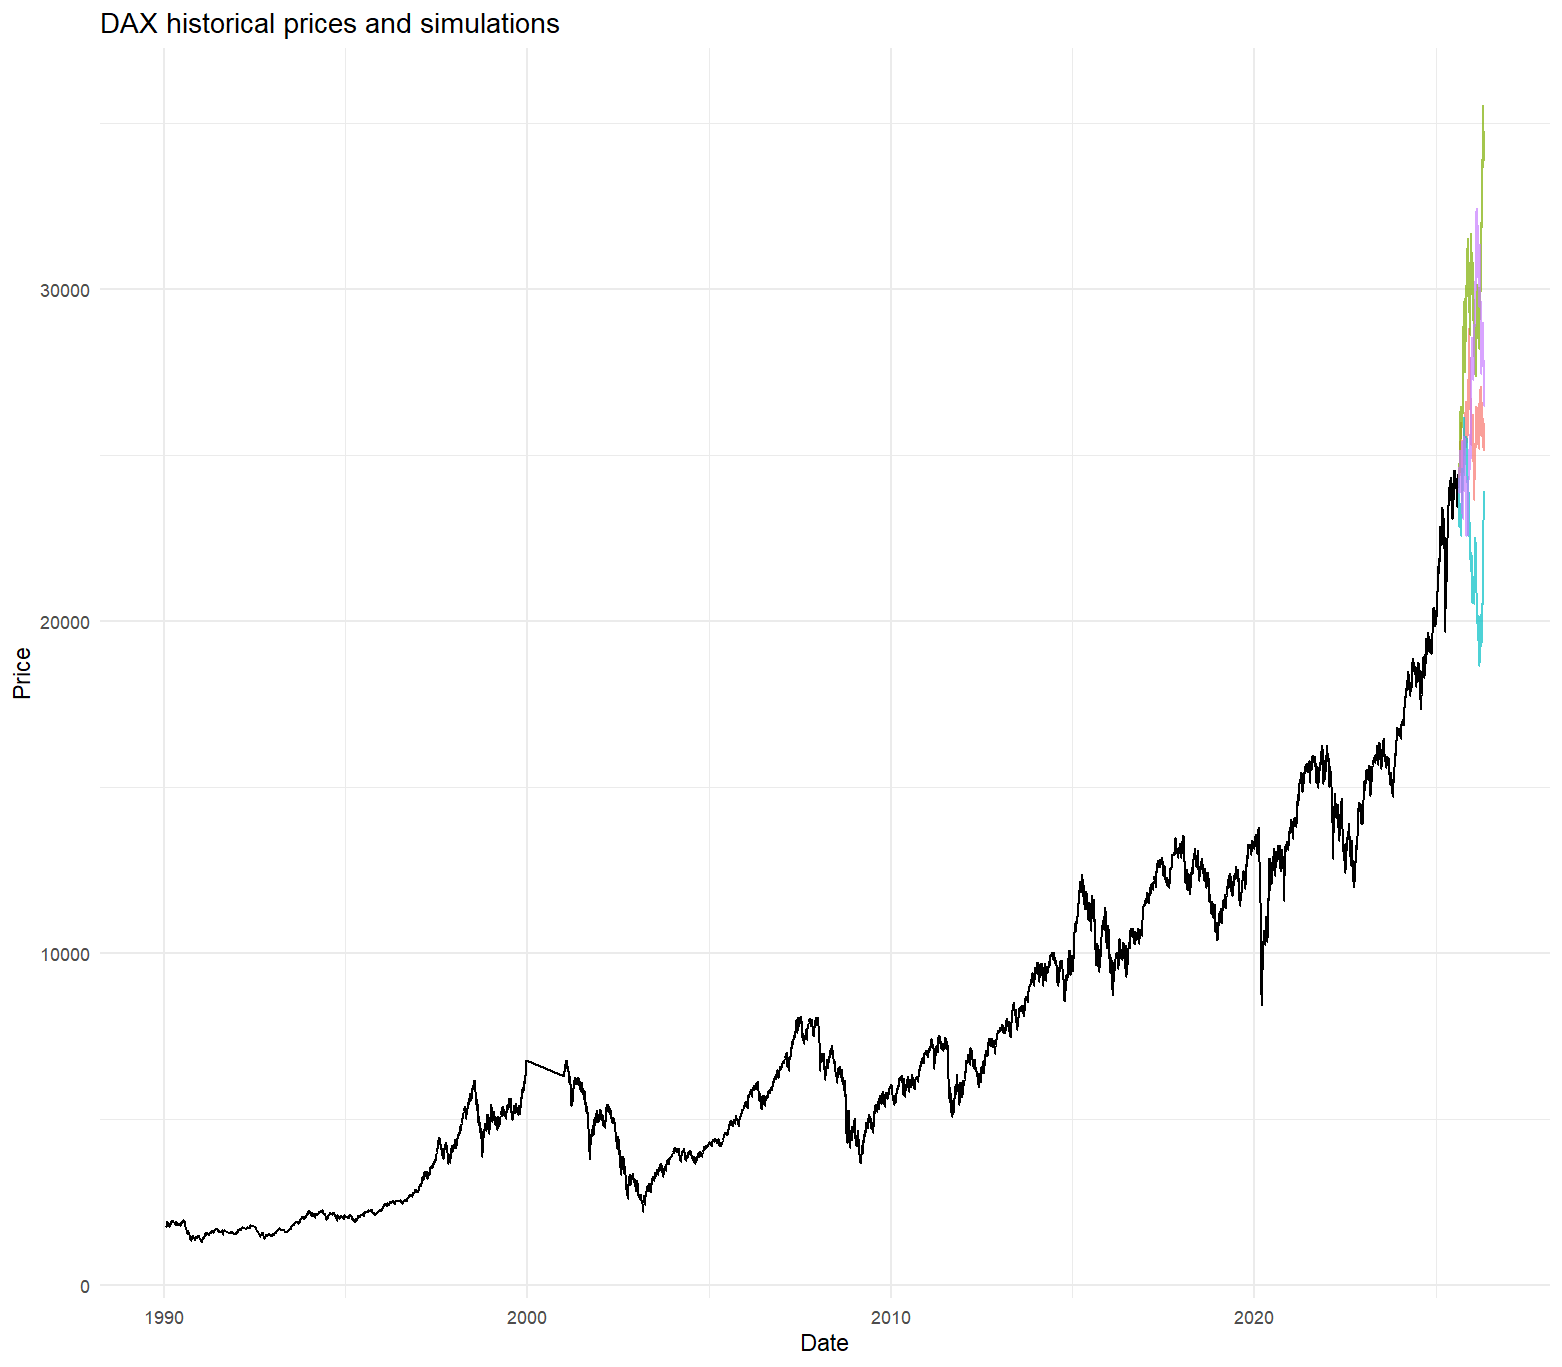
\includegraphics[width=0.8\textwidth]{images/dax_monte_carlo.png}
    \caption{DAX mit 10 simulierten Pfaden für das nächste Jahr}
    \label{fig:dax_monte_carlo}
\end{figure}

\end{bsp}

\begin{bsp}[Vergleich von Konfidenzintervall und Monte-Carlo-Simulation]

Man kann das Konfidenzintervall aus dem vorherigen Beispiel mit den quantilen der Monte-Carlo-Simulation vergleichen.

\begin{figure}[H]
    \centering
    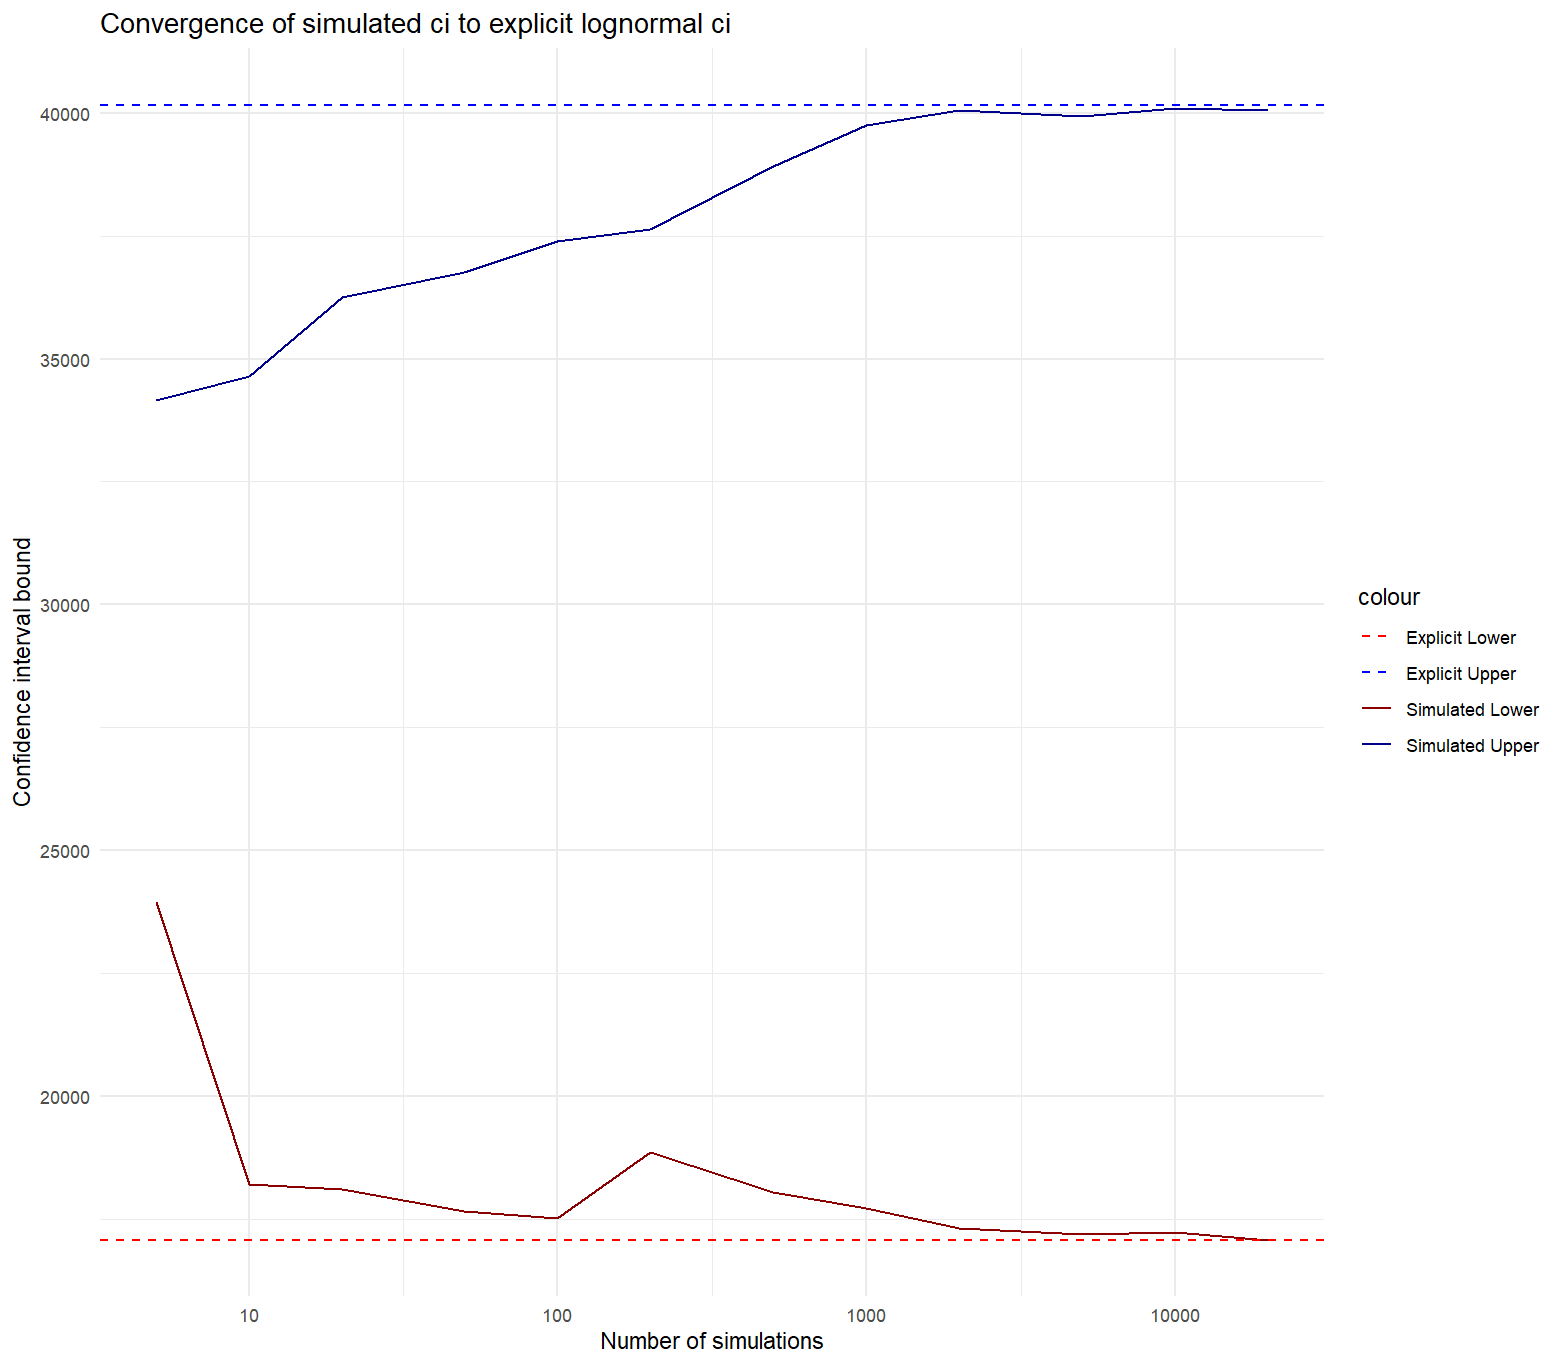
\includegraphics[width=0.9\textwidth]{images/ci_comparison.png}
    \caption{Vergleich von Konfidenzintervall und Monte-Carlo-Simulation für verschiedene Simulationsanzahlen}
    \label{fig:ci_comparison}
\end{figure}
Man erkennt, dass das Konfidenzintervall mit steigender Simulationsanzahl immer besser durch die Quantile der Simulation approximiert wird.
Das spricht für die Korrektheit der beiden Verfahren.

\end{bsp}

\section{Aktienoptionen}

\subsection{Finanzmathematische Grundlagen}

Aktienoptionen sind Finanzderivate, die dem Inhaber das Recht, aber nicht die Pflicht geben, 
eine Aktie zu einem vorher festgelegten Preis (dem Ausübungspreis) zu kaufen (Call-Option) 
oder zu verkaufen (Put-Option). Europäische Optionen können nur am Fälligkeitstag ausgeübt 
werden, während amerikanische Optionen während der gesamten Laufzeit bis zum Verfallsdatum 
ausgeübt werden können. Den fairen Preis einer Option zu bestimmen ist eine Herausforderung,
die man mit Hilfe der geometrischen brownschen Bewegung lösen kann. Im Folgenden wird dazu das Black-Scholes-Modell 
vorgestellt.

\begin{bsp}
\textit{Beispiel Call-Option.} 
Ein Investor erwirbt eine europäische Call-Option auf die Aktie der Firma X mit einem
 Ausübungspreis von 50\,€. Am Fälligkeitstag steht der Aktienkurs bei 60\,€. 
 Der Investor übt die Option aus, kauft die Aktie für 50\,€ und kann 
 sie sofort für 60\,€ verkaufen. Sein Gewinn (ohne Berücksichtigung der Optionsprämie) 
 beträgt 10\,€ pro Aktie.\\
\textit{Motivation.} Der Investor spekuliert darauf, dass der Kurs der Aktie steigt 
und über den Ausübungspreis hinausgeht.

\textit{Beispiel Put-Option.}
Ein Landwirt sichert sich gegen fallende Weizenpreise ab und kauft eine europäische 
Put-Option mit einem Ausübungspreis von 200\,€/Tonne. Am Fälligkeitstag liegt der 
Marktpreis bei 170\,€/Tonne. Der Landwirt übt die Option aus und verkauft seinen 
Weizen zum höheren Preis von 200\,€/Tonne, obwohl der Marktpreis niedriger ist. 
Sein Vorteil beträgt 30\,€ pro Tonne (abzüglich der Optionsprämie).
\end{bsp}
% 
\subsection{Bewertung von Aktienoptionen im Binomialmodell mit dem Risikoneutralem Maß}

Das Binomialmodell wird erweitert. Zusätzlich zur Aktie und deren Kurs gibt es nun die Bank, die einen risikofreien Zinssatz $r$ anbietet.
Zusätzlich wird ein neues Wahrscheinlichkeitsmaß $Q$ eingeführt, das sogenannte risikoneutrale Maß.

\begin{defi}[Arbitrage-Prinzip]
Durch Arbitrage erzielt man Gewinne, in dem man Güter an einem Markt kauft, und dann fast gleichzeitig (teurer) an einem anderen Verkauft.
Die Möglichkeit für Arbitrage existiert nur kurzfristig, da die Preise sich im Weltmarkt ausgleichen. Im vorliegenden Modell wird Arbitrage daher ausgeschlossen.  
Es wird angenommen, dass man keine risikolosen Gewinne erzielen kann, ohne Kapital zu investieren.
\end{defi}

\begin{defi}[Europäische Optionen]
    Europäische Optionen geben dem Inhaber das Recht, 
    einen Basiswert zu einem festgelegten Preis (dem Ausübungspreis) nur am 
    Fälligkeitstag zu kaufen (Call-Option) oder zu verkaufen (Put-Option).
    Der Wert einer europäischen Call-Option am Endzeitpunkt $T$ ist durch die Auszahlungsfunktion
    $$f(S_T) = \max(S_T - K, 0) = (S_T - K)^+$$
    gegeben, wobei $K$ der Ausübungspreis ist. $S_T - K$ ist der Gewinn der erzielt wird, wenn der Inhaber
    Aktien zu einem niedrigeren Kurs ($K$) erwirbt, und dann zum echten Kurs ($S_T$) verkauft.
    Die Auszahlungsfunktion kann keine negativen Werte annehmen, da der Inhaber wohl nicht auf sein Recht bestehen würde, 
    Aktien zu einem erhöhten Kurs zu kaufen. Für eine Put-Option ist die Auszahlungsfunktion
    $$\tilde f(S_T) = \max(K - S_T, 0) = (K - S_T)^+.$$
Das entspricht der \textit{Call-Put-Parität}
    $f(S_T) - \tilde f(S_T) = S_T - K$.
\end{defi}

\begin{defi}[Hedging]
Ein Anbieter von Optionen kann sich absichern, indem er ein sogenanntes 
Hedge-Portfolio bildet. Dieses besteht aus einer dynamischen Position 
im Basiswert sowie einer Position im risikofreien Konto. Ziel ist es, die 
Auszahlungsstruktur der Option durch das Portfolio exakt zu replizieren.  

Formal bedeutet Hedging: Es existieren Prozesse $\Delta_t$ (Anzahl der 
gehaltenen Aktien) und $B_t$ (Bestand im Bankkonto), so dass für alle Zeiten $t$ gilt
\[
V_t = \Delta_t S_t + B_t,
\]
wobei $V_t$ der Wert des Hedge-Portfolios ist. Ist das Portfolio 
selbstfinanzierend, d. h. Änderungen in $V_t$ entstehen ausschließlich 
durch Änderungen in $S_t$ und nicht durch externe Ein- oder Auszahlungen, 
und gilt zudem $V_T = f(S_T)$ mit der Optionsauszahlung $f(S_T)$, 
so spricht man von einer perfekten Replikation. Die Grundidee wird am Beispiel einer europäischen Call-Option verdeutlicht: Steigt der Wert der Aktie über den Ausübungspreis $K$ und der Optionsanbieter ist verpflichtet, die Aktie zum Preis $K$ zu liefern, so können dafür die im Hedge-Portfolio gehaltenen Aktien verwendet werden. Auf diese Weise wird der potenzielle Verlust ausgeglichen.
\end{defi}


\begin{bem}[Risikoneutrale Wahrscheinlichkeit für einen Schritt]\label{bem:q_prob_1_step}
Ein Betrag $B_0$ der aus dem Bankkonto angelegt wird steigt durch den risikofreien Zinssatz $r$ kontinuierlich durch
$$B(t) = e^{rt}B_0.$$
Daher ist ein Gewinn in der Zukunft ($\Delta t$) weniger wert als ein Gewinn jetzt, da man den jetzigen Gewinn $G$ anlegen könnte, und 
dann $Ge^{r \Delta t}$ hätte. 

Da die dies berücksichtigt werden muss,
werden mögliche Aktiengewinne mit dem Faktor $e^{r \Delta t}$ verkleinert (diskontiert).

Der diskontierte Aktienkurs zum Zeitpunkt $n$ ist $e^{-r n \Delta t} S_n$.
Im Folgenden wird berechnet, für welche Wahrscheinlichkeit der neue diskontierte Prozess
ein Martingal ist. Das Martingal-Kriterium lautet: $E(X_{n+1} \mid X_n = l) = l$, wobei $X_n = e^{-r n \Delta t} S_n$.
Einsetzen von $X_{n+1} = e^{-r (n+1) \Delta t} S_{n+1}$ und $X_n = e^{-r n \Delta t} S_n$ ergibt
$$
E(e^{-r (n+1) \Delta t} S_{n+1} \mid S_n = v) = e^{-r n \Delta t} v
$$
Aus der Linearität des Erwartungswerts folgt
$$
E(e^{-r \Delta t} S_{n+1} \mid S_n=v) = v.
$$
Setzt man die möglichen Werte für $S_{n+1}$ ein ($S_{n+1} = u S_n$ mit Wahrscheinlichkeit $q$, $S_{n+1} = d S_n$ mit Wahrscheinlichkeit $1-q$) folgt
$$
e^{-r \Delta t} \left( q u S_n + (1-q) d S_n \right) = v.
$$
Teilt man durch $S_n = v$ ($v > 0$) ergibt sich
$$
e^{-r \Delta t} \left( q u + (1-q) d \right) = 1.
$$
Das ist äquivalent zu
$$
q = \frac{e^{r \Delta t} - d}{u - d}.
$$
Zum Vergleich: im klassischen Binomialmodell ist 
$$p = \frac{1 - d}{u - d}$$
die „risikoneutrale Wahrscheinlichkeit“. Anders als zuvor
wurde aber lediglich eine schwächere Aussage gezeigt (nur ein Schritt). 
Das wird am Folgenden jedoch nachgezogen.

\end{bem}

\begin{defi}[Risikoneutrales Maß]
Die soeben berechnete Wahrscheinlichkeit $q$ gehört zum risikoneutralen Wahrscheinlichkeitsmaß $Q$.
Bisher wurde mit dem ursprünglichen Maß $P$ gerechnet. Ab jetzt wird mit $E(X)$, $V(X)$ etc der Erwartungswert
und die Varianz unter $P$ bezeichnet, während $E_Q(X)$, $V_Q(X)$ etc den Erwartungswert und die Varianz unter $Q$
bezeichnen. An $Q$ werden folgende Anforderungen gestellt (vgl. \cite{hull}, S. 270):
\begin{enumerate}
    \item $Q$ ist ein Wahrscheinlichkeitsmaß
    \item $Q$ ist äquivalent zu $P$, das heißt $P(A)=0 \iff Q(A)=0$ für alle Ereignisse $A$ (lediglich die Wahrscheinlichkeiten ändern sich, nicht die möglichen Ereignisse)
    \item Unter $Q$ ist der diskontierte Aktienkurs ein Martingal, also $$E_Q(e^{-r \Delta t} S_{t} \mid S_s = v) = e^{-rs\Delta t}\, v$$ für alle $t \gt s$ und $v>0$.
\end{enumerate}
Im Fall des Binomialmodells handelt es sich um ein diskretes Wahrscheinlichkeitsmaß, 
wobei die Werte $Q(S_{t + \Delta t} = u \cdot S_t)=q$ und $Q(S_{t + \Delta t} = d \cdot S_t)=1-q$ bekannt sind.
Oft können Maße in der Stochastik nur indirekt über ihre Eigenschaften definiert werden, das gilt auch hier. Die Untersuchung der Existenz und Eindeutigkeit eines solchen Maßes überschreitet den Rahmen dieser Arbeit; Es sei auf Shreve \cite{shreve}, (2004, Kap. 5) verwiesen.
\end{defi}

\begin{lemma}[Martingal-Eigenschaft des diskontierten Aktienkurses unter $Q$]
Mit der Schrittwahrscheinlichkeit aus der Bemerkung \ref{bem:q_prob_1_step} wird nachgewiesen,
dass der diskontierte Aktienkurs unter dem risikoneutralen Maß $Q$ ein Martingal ist. Dies ergibt sich zwar aus den Anforderungen 
an $Q$, kann aber mit der Ein-Schritt-Übergangswahrscheinlichkeit verifiziert werden.
Setze $X_n := e^{-r n \Delta t}\, S_n$. Unter dem risikoneutralen Maß $Q$, das heißt für 
$q=\frac{e^{r\Delta t}-d}{u-d}$ ist $(X_n)_{n\in\mathbb N_0}$ ein Martingal.

\textit{Beweis.} Schreibe $S_{n+1}=S_n\,\xi_{n+1}$ mit 
$Q(\xi_{n+1}=u)=q$ und $Q(\xi_{n+1}=d)=1-q$. 
Für $s<t$ beliebig und wegen Unabhängigkeit der Schritte:
$$
X_t
= e^{-rt\Delta t} S_t
= e^{-rt\Delta t} S_s \prod_{i=s+1}^{t} \xi_i,
$$
also
$$
\begin{aligned}
E_Q(X_t\mid S_s=v)
&= e^{-rt\Delta t}\, v \prod_{i=s+1}^{t} E_Q(\xi_i)
= e^{-rt\Delta t}\, v \big(q u + (1-q)d\big)^{t-s} \\
&= e^{-rt\Delta t}\, v \big(e^{r\Delta t}\big)^{t-s}
= e^{-rs\Delta t}\, v
\end{aligned}
$$
Damit ist $(X_n)$ ein Martingal. \qed
\end{lemma}

\begin{satz}[Bewertung von europäischen Optionen im Binomialmodell]
Der Preis einer Option durch rekursive Rückwärtsinduktion bestimmt. 
Der Wert einer europäischen Option am Endzeitpunkt $T$ ist durch die Auszahlungsfunktion $f(S_T)$ gegeben, z.\,B.\ für eine Call-Option $f(S_T) = \max(S_T - K, 0)$.
Die Bewertung zu früheren Zeitpunkten erfolgt rekursiv rückwärts:
$$
\begin{aligned}
C_n &= e^{-r \Delta t} \left( q C_{n+1}^\text{up} + (1-q) C_{n+1}^\text{down} \right) \\
&= E_Q(e^{-r \Delta t} C_{n+1} \mid S_n)
\end{aligned}
$$
wobei $C_{n+1}^\text{up}$ und $C_{n+1}^\text{down}$ die Optionswerte im nächsten Schritt nach Auf- bzw. Abbewegung sind.
Damit lässt sich der Optionspreis am Anfangszeitpunkt $C_0$ bestimmen. Die Formel leitet
sich aus dem Ewartungswert unter dem risikoneutralen Maß $Q$ ab, dessen Verhalten im ein-stufigen Fall ja explizit bekannt ist.
Der faire Preis der Option ist der Erwartungswert der diskontierten Auszahlung.
\end{satz}

\begin{bsp}
Seien $S_0 = 100\,€$, $u=1.2$, $d=0.8$, $r=0.05$, $\Delta t=1$ Jahr, $K=100\,€$ und $T=2$ Jahre.
Die risikoneutrale Wahrscheinlichkeit ist $q = \frac{e^{0.05}-0.8}{1.2-0.8} \approx 0.628$.
Die möglichen Aktienkursentwicklungen zum Zeitpunkt $T$ werden in Abbildung \ref{fig:binomialtree_options} gezeigt:
\begin{figure}[H]
\centering
\begin{tikzpicture}[x=3.2cm,y=1.4cm,>=stealth]
    % styles
    \tikzset{price/.style={circle,draw,minimum size=6mm,inner sep=0pt,font=\small}}
    % nodes
    \node[price] (S0)  at (0,0)   {100};
    \node[price] (Su)  at (1,1)   {120};
    \node[price] (Sd)  at (1,-1)  {80};
    \node[price] (Suu) at (2,2)   {144};
    \node[price] (Sud) at (2,0)   {96};
    \node[price] (Sdd) at (2,-2)  {64};

    % edges with risk-neutral probabilities
    \draw[->] (S0) -- node[sloped,above] {$p$} (Su);
    \draw[->] (S0) -- node[sloped,below] {$1-p$} (Sd);

    \draw[->] (Su) -- node[sloped,above] {$p$} (Suu);
    \draw[->] (Su) -- node[sloped,below] {$1-p$} (Sud);

    \draw[->] (Sd) -- node[sloped,above] {$p$} (Sud);
    \draw[->] (Sd) -- node[sloped,below] {$1-p$} (Sdd);

    % time axis labels
    \node[font=\scriptsize] at (0,-2.4) {Zeit 0};
    \node[font=\scriptsize] at (1,-2.4) {Zeit 1};
    \node[font=\scriptsize] at (2,-2.4) {Zeit 2 = T};

    % parameter box
    \node[anchor=west, align=left, font=\scriptsize] at (2.6,2.0) {Parameter:\\
        $u=1.2,\; d=0.8$\\
        $r=0.05,\; \Delta t=1$\\
        $q \approx 0.628$ \\
        $p \ \ \mathrm{beliebig}$
    };
\end{tikzpicture} 
\caption{Kursentwicklung mit Binomialmodell}
\label{fig:binomialtree_options}
\end{figure}
Die Auszahlungen der Call-Option zum Zeitpunkt $T$ sind:
$$
\begin{aligned}
C_{T,\text{up}} &= \max(144 - 100, 0) = 44\,€, \\
C_{T,\text{mid}} &= \max(96 - 100, 0) = 0\,€, \\
C_{T,\text{down}} &= \max(64 - 100, 0) = 0\,€.
\end{aligned}
$$
Rückwärtsinduktion:
$$
\begin{aligned}
C_{1,\text{up}} &= e^{-0.05} \left( q \cdot 44 + (1-q) \cdot 0 \right) \approx 26.28\,€, \\
C_{1,\text{down}} &= e^{-0.05} \left( q \cdot 0 + (1-q) \cdot 0 \right) = 0\,€, \\
C_0 &= e^{-0.05} \left( q \cdot 23.99 + (1-q) \cdot 0 \right) \approx 15.7\,€.
\end{aligned}
$$
Der faire Preis der Call-Option ist also etwa 15.7\,€.
\end{bsp}

\subsection{Das Black-Scholes-Modell als Grenzfall des Binomialmodells}
Ziel ist es zu zeigen, dass die fairen Optionspreise
beim Verfeinern der Zeitdiskretisierung gegen die geometrische brownsche Bewegung konvergieren.
Dieses Modell wird auch als Black-Scholes-Modell bezeichnet. Hier wird der Grenzübergang im risikoneutralen Maß durchgeführt.
Die Modellannahme aus Kapitel 4 wird übernommen:
$$
S_t = S_0 \cdot e^{(\mu - \frac{1}{2}\sigma^2)t + \sigma W_t}
$$
und durch Zeitdiskretisierung:
$$
S_{t+\Delta t} = S_t \cdot e^{(\mu - \frac{1}{2}\sigma^2)\Delta t + \sigma W_{t+\Delta t}}.
$$

\begin{satz}[das erweiterte Binomialmodell unter dem Risikoneutralen Maß]
Unter $Q$ entspricht der Optionspreis der geometrischen Brownschen Bewegung mit den Parametern $r$ (Rendite)
und $\sigma$ (Volatilität der Aktie).


\textit{Beweis}. Zur Vereinfachung der zeitdiskreten Sprunggrößen $u$ und $d$ wird der Drift vernachlässigt.
Das wird durch ein Arbitrage-Argument gerechtfertigt (vgl. Behrends\cite{behrends}, S. 133):
Der deterministische Teil der Preisbewegung muss unter dem risikoneutralen Maß verschwinden, 
sonst gäbe es eine risikolose Gewinnmöglichkeit (Arbitrage). 
Für einen Zeitschritt $\Delta t$ folgen damit die Sprunggrößen
$$
u = e^{\sigma \sqrt{\Delta t}},\quad d = e^{-\sigma \sqrt{\Delta t}}
$$
und den risikoneutralen Schritt $q(\Delta t)$ aus dem Martingal-Kriterium
$$
q(\Delta t) = \frac{e^{r \Delta t} - d}{u - d}
= \frac{e^{r \Delta t} - e^{-\sigma \sqrt{\Delta t}}}{e^{\sigma \sqrt{\Delta t}} - e^{-\sigma \sqrt{\Delta t}}}.
$$
\\ Durch eine Taylor-Entwicklung um $0$ werden die Funktionen wieder vereinfacht. Analog zum Beweis aus Kapitel 4
sollen höhere Potenzen von $\Delta t$ im Grenzwert verschwinden. Da es sich um einen Quotienten handelt,
kann man die Abschätzung aber nicht direkt anwenden. Stattdessen werden Zähler und Nenner separat entwickelt:
$$
e^{r\Delta t} = 1 + r\Delta t + o(\Delta t),\quad
e^{\pm \sigma\sqrt{\Delta t}} = 1 \pm \sigma \sqrt{\Delta t} + \tfrac12 \sigma^2 \Delta t + o(\Delta t).
$$
Damit
$$
\begin{aligned}
\text{Zähler} &= e^{r \Delta t} - e^{-\sigma \sqrt{\Delta t}}
= \big(1 + r\Delta t + o(\Delta t)\big) - \big(1 - \sigma \sqrt{\Delta t} + \tfrac12 \sigma^2 \Delta t + o(\Delta t)\big) \\
&= \sigma \sqrt{\Delta t} + \big(r - \tfrac12 \sigma^2\big)\Delta t + o(\Delta t), \\
\text{Nenner} &= e^{\sigma \sqrt{\Delta t}} - e^{-\sigma \sqrt{\Delta t}}
= \big(1 + \sigma \sqrt{\Delta t} + \tfrac12 \sigma^2 \Delta t + o(\Delta t)\big) \\
&\qquad\qquad\qquad - \big(1 - \sigma \sqrt{\Delta t} + \tfrac12 \sigma^2 \Delta t + o(\Delta t)\big)
= 2\sigma \sqrt{\Delta t} + o(\sqrt{\Delta t}).
\end{aligned}
$$
Insgesamt:
$$
q(\Delta t) = \frac{\sigma \sqrt{\Delta t} + \big(r - \tfrac12 \sigma^2\big)\Delta t + o(\Delta t)}{2\sigma \sqrt{\Delta t} + o(\sqrt{\Delta t})}
= \tfrac12 + \frac{r - \tfrac12 \sigma^2}{2\sigma}\,\sqrt{\Delta t} + o(\sqrt{\Delta t}).
$$
An dieser Stelle ist wichtig, dass die Anzahl der Schritte $N_u$ in denen die Aktie steigt, binomialverteilt ist.
Und zwar zur Anzahl der Schritte $n=T/\Delta t$ mit festen Wahrscheinlichkeit $q(\Delta t)$.
Dann gilt
$$
S_T^{(n)} = S_0\, u^{N_u}\, d^{n-N_u}
= S_0 \exp\!\big(\sigma \sqrt{\Delta t}\,(2N_u - n)\big).
$$
Und somit
$$
\log S_T^{(n)}
= \log S_0 + \sigma \sqrt{\Delta t}\,(2N_u - n).
$$
Es wird eine 0 addiert:
$$
2N_u - n
= 2\big(N_u - n q(\Delta t)\big) + n\big(2q(\Delta t)-1\big).
$$
Zwischenfazit:
$$
\log S_T^{(n)}
= \log S_0 + \sigma \sqrt{\Delta t}\, n\big(2q(\Delta t)-1\big)
+ \sigma \sqrt{\Delta t}\, 2\big(N_u - n q(\Delta t)\big).
$$
Zuerst wird der stochastische Term (rechts) untersucht: Da die Binomialverteilung eine Summe von unabhängigen Bernoulli-Verteilungen ist, kann der zentrale Grenzwertsatz angewendet werden:
$$
\lim_{n\to\infty} N_u = \lim_{n \to \infty} \sum_{k=0}^{n}\text{Ber}(q(\Delta t)) \sim \mathcal N\big(n q(\Delta t), n q(\Delta t)(1-q(\Delta t))\big).
$$
Das ist äquivalent zu
$$
\frac{N_u - n q(\Delta t)}{\sqrt{n\,q(\Delta t)(1-q(\Delta t))}} \longrightarrow Z\sim \mathcal N(0,1),
$$
also
$$
2\big(N_u - n q(\Delta t)\big) = 2\sqrt{n\,q(\Delta t)(1-q(\Delta t))}\,Z_n,
$$
wobei $Z_n\longrightarrow Z$.
Schließlich folgt aus $q(\Delta t)\to \tfrac12$ für $\Delta t\to 0$:
$$
\begin{aligned}
\sigma \sqrt{\Delta t}\cdot 2\sqrt{n\,q(\Delta t)(1-q(\Delta t))}\,Z_n
&= 2\sigma \sqrt{n\Delta t}\,\sqrt{q(\Delta t)(1-q(\Delta t))}\,Z_n \\
&= 2\sigma \sqrt{T}\,\sqrt{\tfrac14 + o(1)}\,Z_n
= \sigma \sqrt{T}\,Z_n + o(1).
\end{aligned}
$$
Nun wird der deterministische Term (mittig) untersucht:
\\ Multipliziere mit $\sigma \sqrt{\Delta t}$ und benutze $n\Delta t=T$ sowie $q(\Delta t)=\tfrac12 + \alpha \sqrt{\Delta t} + o(\sqrt{\Delta t})$ mit
$\alpha=\frac{r-\frac12\sigma^2}{2\sigma}$:
$$
\begin{aligned}
\sigma \sqrt{\Delta t}\, n\big(2q(\Delta t)-1\big)
&= \sigma \sqrt{\Delta t}\, n\big(2\alpha \sqrt{\Delta t} + o(\sqrt{\Delta t})\big)
= \sigma\, n \big(2\alpha \Delta t + o(\Delta t)\big) \\
&= \sigma \cdot 2\alpha \cdot (n\Delta t) + o(1)
= \big(r - \tfrac12 \sigma^2\big)T + o(1).
\end{aligned}
$$
Zwischenfazit:
$$
\log S_T^{(n)}
= \log S_0 + \big(r - \tfrac12 \sigma^2\big)T + \sigma \sqrt{T}\,Z_n + o(1).
$$
Im Grenzwert $n\to\infty$ (bzw.\ $\Delta t \to 0$) folgt damit
$$
\log S_T \sim \mathcal N\!\Big(\log S_0 + \big(r - \tfrac12 \sigma^2\big)T,\;\sigma^2 T\Big),
$$
d.\,h.\ unter $Q$ konvergiert der diskrete Prozess gegen die geometrische brownsche Bewegung. Der Drift-Term ist nicht mehr der
Trend im Aktienkurs sondern der Zinssatz $r$.
\qed
\end{satz}

\begin{satz}[Black–Scholes-Formel für europäische Call-Optionen]
Sei $C_0^{(n)}$ der Preis der europäischen Call-Option mit Laufzeit $T$ und Strike $K$
im $n$-stufigen Binomialmodell unter Diskontierung mit $r$. Dann gilt
$$
\lim_{n\to\infty} C_0^{(n)}
= C_0^{\mathrm{BS}}
= S_0\,\Phi(d_1) - K e^{-rT}\,\Phi(d_2),
$$
wobei
$$
d_1 = \frac{\ln(S_0/K) + \big(r + \tfrac12 \sigma^2\big)T}{\sigma \sqrt{T}},
\qquad
d_2 = d_1 - \sigma \sqrt{T},
$$
und $\Phi$ die Verteilungsfunktion der Standardnormalverteilung ist.
\\ \textit{Beweis}\footnote{Der Beweis ist angelehnt an die Argumentation in Hull, 2022 \cite{hull}, S. 347}. Risikoneutrale Bewertung im Binomialmodell liefert
$$
C_0^{(n)} = e^{-rT}\,E_Q\!\left[(S_T^{(n)} - K)^+\right].
$$
Die obige Verteilungskonvergenz impliziert
$$
S_T^{(n)} \longrightarrow S_T = S_0 \exp\!\big((r-\tfrac12\sigma^2)T + \sigma \sqrt{T}\,Z\big).
$$
Nun wird der Satz von Pratt (s. Anhang) angewendet, um den Grenzübergang und den Erwartungswert zu vertauschen. Eine untere Schranke ist $Y_n=0$ und eine obere Schranke ist $Z_n = (S_T^{(n)})^+ = S_T^{(n)}$. 
$$
\lim_{n\to\infty} C_0^{(n)} = e^{-rT}\,E_Q\!\left[ (\lim_{n\to\infty} S_T^{(n)}-K)^+ \right] = e^{-rT}\,E_Q\!\left[(S_T - K)^+\right].
$$
Nun wird die rechte Seite explizit berechnet: Seien
$$
m := \big(r-\tfrac12\sigma^2\big)T,\qquad v:=\sigma \sqrt{T},\qquad Z\sim \mathcal N(0,1),
$$
also $S_T = S_0 e^{m + v Z}$. Dann gilt
$$
E_Q\big[(S_T - K)^+\big]
= E_Q\big[S_T\,\mathbf 1_{\{S_T\ge K\}}\big] - K\,Q(S_T\ge K).
$$
Aus Kapitel 4 ist bekannt, das $S_T$ lognormalverteilt ist. Die Schranke $S_T\ge K$ ist daher äquivalent zu $m + vZ \ge \ln(K/S_0)$, also
$$
Z \ge a := \frac{\ln(K/S_0) - m}{v}.
$$
Damit ergibt sich für den zweiten Term
$$
Q(S_T\ge K) = Q(Z\ge a) = \Phi(-a).
$$
Für den ersten Term wird die Dichte $\varphi$ von $Z$ genutzt:
$$
\begin{aligned}
E_Q\big[S_T\,\mathbf 1_{\{Z\ge a\}}\big]
&= S_0 e^{m}\int_a^\infty e^{v x}\,\varphi(x)\,dx
= S_0 e^{m}\int_a^\infty e^{v x}\,\frac{1}{\sqrt{2\pi}}e^{-x^2/2}\,dx \\
&= S_0 e^{m}\int_a^\infty \frac{1}{\sqrt{2\pi}}
\exp\!\Big(-\tfrac12(x^2 - 2 v x)\Big)\,dx \\
&= S_0 e^{m}\int_a^\infty \frac{1}{\sqrt{2\pi}}
\exp\!\Big(-\tfrac12(x - v)^2 + \tfrac12 v^2\Big)\,dx \\
&= S_0 e^{m + \frac12 v^2}\int_a^\infty \varphi(x - v)\,dx.
\end{aligned}
$$
Mit der Substitution $y=x-v$ folgt
$$
\int_a^\infty \varphi(x - v)\,dx = \int_{a-v}^\infty \varphi(y)\,dy = \Phi(v-a).
$$
Der zweite Term ist damit bestimmt:
$$
E_Q\big[S_T\,\mathbf 1_{\{S_T\ge K\}}\big]
= S_0 e^{m + \frac12 v^2}\,\Phi(v-a).
$$
Zwischenfazit:
$$
E_Q\big[(S_T - K)^+\big] = S_0 e^{rT}\,\Phi(d_1) - K\,\Phi(d_2)
$$
Setze $m+\tfrac12 v^2 = rT$ und beachte
$$
v-a = \frac{\ln(S_0/K) + (r+\tfrac12\sigma^2)T}{\sigma \sqrt{T}} = d_1,
\qquad
-a = \frac{\ln(S_0/K) + (r-\tfrac12\sigma^2)T}{\sigma \sqrt{T}} = d_2.
$$
Damit gilt
$$
E_Q\big[(S_T - K)^+\big]
= S_0 e^{rT}\,\Phi(d_1) - K\,\Phi(d_2),
$$
und folglich
$$
C_0^{\mathrm{BS}} = e^{-rT}\,E_Q\big[(S_T - K)^+\big]
= S_0\,\Phi(d_1) - K e^{-rT}\,\Phi(d_2).
$$
\qed
\end{satz}

\begin{bem}
Für den europäischen Put folgt analog
$$
P_0^{\mathrm{BS}} = K e^{-rT}\,\Phi(-d_2) - S_0\,\Phi(-d_1),
$$
oder per Put-Call-Parität.

\end{bem}

\begin{bsp}[Call-Option auf den DAX]
Mit der zuvor geschätzten Volatilität ($\sigma$) des DAX kann
man nun den Preis einer Call-Option auf den DAX berechnen. Das folgende
R-Programm (Ausschnitt) berechnet den Preis einer Call-Option abhängig
vom Ausübungspreis $K$.

\begin{lstlisting}
d1 <- (log(S0/K) + (r + 0.5 * sigma^2) * T) / (sigma * sqrt(T))
d2 <- d1 - sigma * sqrt(T)
C <- S0 * pnorm(d1) - K * exp(-r*T) * pnorm(d2)
\end{lstlisting}
Ein Beispiel mit $r = 0.02, T = 1$ Jahr und dem DAX-Stand $S_0 = 24290$ wird in
der folgenden Grafik dargestellt. Der faire Preis der Option
fällt (erwartungsgemäß) mit dem Ausübungspreis $K$.
Aus der Call-Put-Parität folgt, dass der Preis einer Put-Option
sich durch

\begin{lstlisting}
P <- C - S0 + K * exp(-r * T)
\end{lstlisting}
berechnet.

\begin{figure}[H]
    \centering
    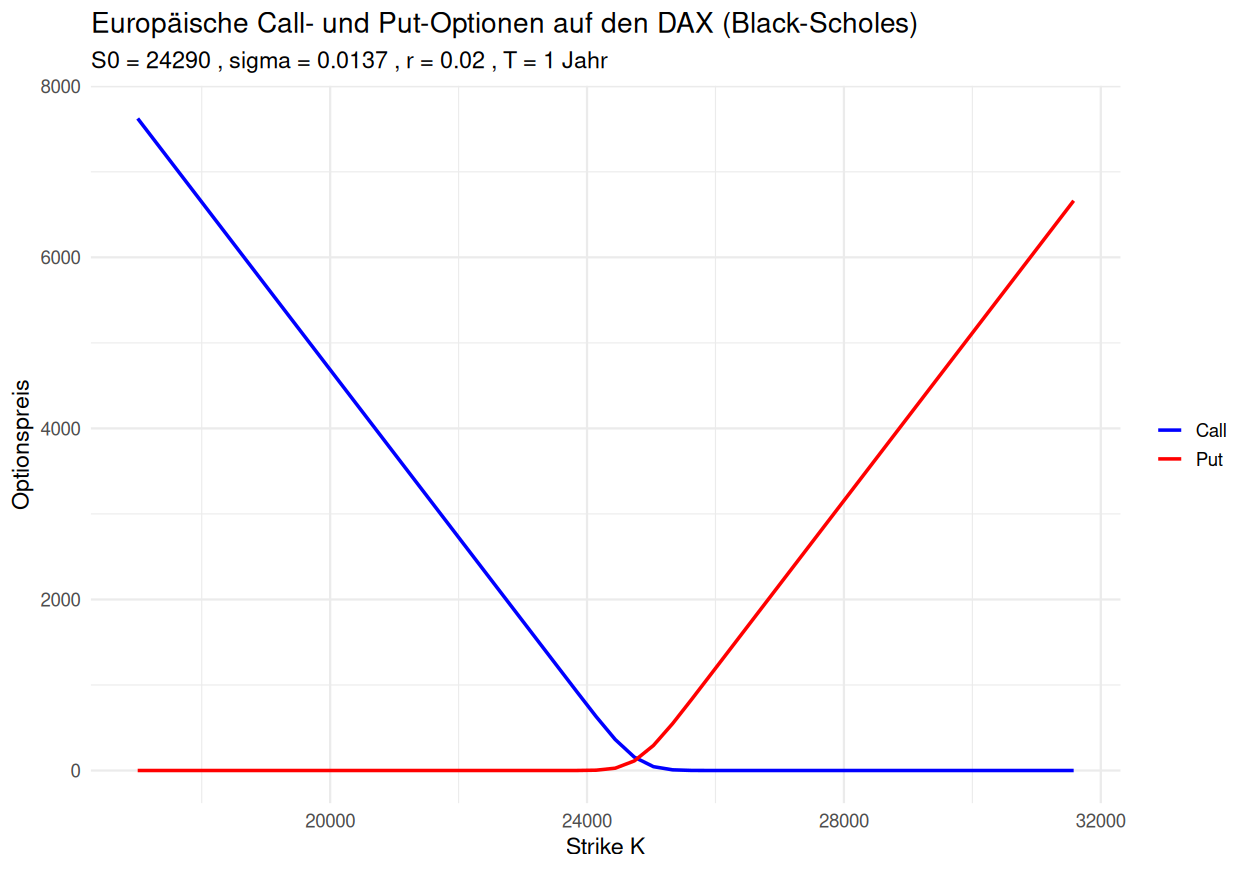
\includegraphics[width=0.9\textwidth]{images/dax_bs.png}
    \caption{Preis einer Call-Option der entsprechenden Put-Option auf den DAX in Abhängigkeit vom Ausübungspreis $K$}
    \label{fig:dax_bs}
\end{figure}

\end{bsp}

\subsection{Bewertung von Aktienoptionen mit Monte-Carlo-Verfahren}
Der letzte Beweis zeigt, dass explizite Formeln für Optionspreise nur mit hohem
Aufwand hergeleitet werden können. Man bedenke, dass es sich um eine 
vergleichsweise simple Option gehandelt hat. Für komplexere Derivate
gibt es meist keine geschlossenen Formeln. Stattdessen werden numerische Verfahren
verwendet, um den Erwartungswert der diskontierten Auszahlung zu approximieren.


\begin{lemma}[Anwendung auf Optionspreise]
Um allgemeine Optionen zu bewerten, muss die Auszahlungsfunktion $f$
nicht bloß relle Zahlen auf relle Zahlen abbilden, sondern des gesamten Pfad
$S_t$, $t\in[0,T]$ auf reelle Zahlen Abbilden. Bei z. B. asiatischen Optionen ist
der Durchschnittskurs über die Laufzeit relevant.
Sei also im Folgenden 
$$f: C([0,T]) \to \mathbb R, \tilde S_T \mapsto f(\tilde S_T)$$
eine Auszahlungsfunktion. Der faire Option mit Auszahlung $f(S_T)$
unter dem risikoneutralen Maß $Q$ ist
$$
C_0 = e^{-rT} E_Q[f(S_T)].
$$
Der Monte-Carlo-Schätzer (s. Anhang) für $C_0$ ist somit
$$
\hat{C}_0^{(n)} = e^{-rT} \frac{1}{n} \sum_{i=1}^n f(S_T^{(i)}),
$$
wobei $S_T^{(i)}$, $i=1,\ldots,n$ unabhängige Realisierungen des Prozesses $S_T$ sind. Aus Kapitel 6 ist
ein Algorithmus bekannt, um Realisierungen der geometrischen brownschen Bewegung $S_T$ zu erzeugen.

\end{lemma}

\begin{bsp}[Monte-Carlo-Simulation einer Call-Option auf den DAX]

Das folgende R-Programm simuliert den Preis einer Call-Option auf den DAX
mit dem Monte-Carlo-Verfahren. Dabei wird die geometrische brownsche Bewegung
simuliert und der Erwartungswert der diskontierten Auszahlung approximiert.

\begin{lstlisting}
  Z <- rnorm(n)
  ST <- S0 * exp((r - 0.5*sigma^2)*T + sigma*sqrt(T)*Z)
  payoff <- pmax(ST - K, 0) # Bewertungsfunktion
  C <- exp(-r*T) * mean(payoff)
\end{lstlisting}
Nun wird der simulierte Preis mit dem Preis aus der Black-Scholes-Formel verglichen. 
Die folgende Grafik zeigt den Vergleich für verschiedene Ausübungspreise $K$.
Je höher die Anzahl der Simulationen $n$, desto genauer ist die Approximation.

\begin{figure}[H]
    \centering
    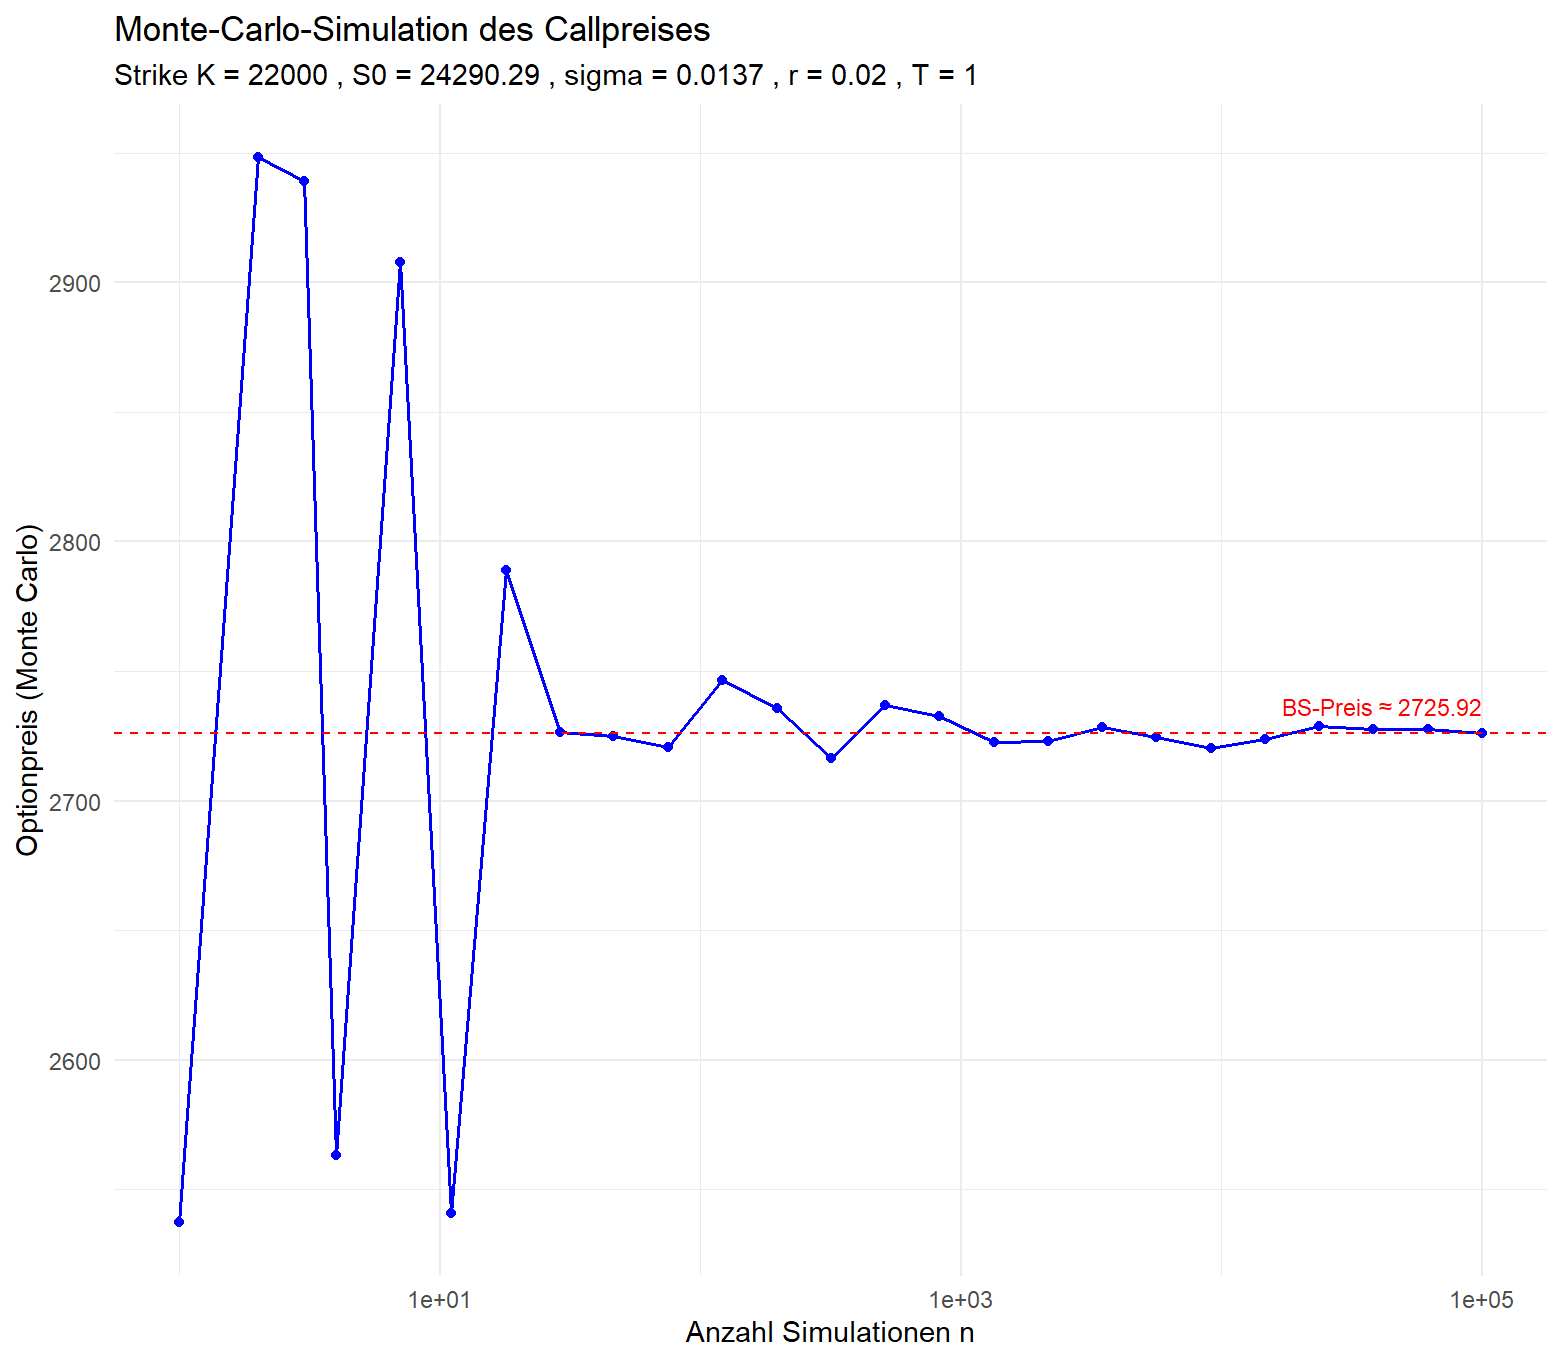
\includegraphics[width=0.9\textwidth]{images/call_dax_mc.png}
    \caption{Preis einer Call-Option auf den DAX in Abhängigkeit der Simulationsanzahl $n$ im Vergleich zur Black-Scholes-Formel}
    \label{fig:call_dax_mc}
\end{figure}

\end{bsp}

\begin{bsp}[Asiatische Optionen]
Asiatische Optionen sind Finanzderivate, bei denen die Auszahlung auf dem Durchschnittspreis
des Basiswerts über einen bestimmten Zeitraum basiert, anstatt auf dem Preis zu einem einzigen Zeitpunkt.
Die Auszahlung einer asiatischen Call-Option mit Ausübungspreis $K$ und Laufzeit $T$ ist
$$f(S_T) = \max\left(\frac{1}{T} \int_0^T S_t\,dt - K, 0\right).$$
Die Bewertung erfolgt mit dem Monte-Carlo-Verfahren, da in dieser Arbeit keine geschlossene Formel wie bei der Black-Scholes vorliegt.
Die Implementierung in R könnte wie folgt aussehen:

\begin{lstlisting}
Z <- matrix(rnorm(N * m), nrow=N, ncol=m) # N Pfade mit m Zeitschritten
dt <- T / m
S <- matrix(0, nrow=N, ncol=m)
S[,1] <- S0
for (j in 2:m) {
  S[,j] <- S[,j-1] * exp((r - 0.5*sigma^2)*dt + sigma*sqrt(dt)*Z[,j])
}
avg_price <- rowMeans(S) # Durchschnittspreis für jeden Pfad
payoff <- pmax(avg_price - K, 0) # Bewertungsfunktion
C <- exp(-r*T) * mean(payoff) # diskontierter Monte-Carlo-Schätzer
\end{lstlisting}

\end{bsp}

\newpage

\section{Fazit}

Die Arbeit spannte den Bogen von elementaren stochastischen Prozessen über das Binomialmodell und die diskrete Brownsche 
Bewegung bis zur geometrischen Brownschen Bewegung als kontinuierlichem Grenzfall. Zentrale stochastische Begriffe wie 
Filtration, bedingter Erwartungswert und Martingal wurden eingeführt und in diskreten Wahrscheinlichkeitsräumen verankert. 
Durch Grenzwertbetrachtungen werden die Konzepte dann auf kontinuierliche Wahrscheinlichkeitsräume übertragen. Über eine 
Logarithmierung und eine systematische Taylor-Approximation der diskreten Renditen wurde gezeigt, dass im Grenzübergang 
$\Delta t \to 0$ die Kursdynamik durch
$S_T = S_0 \exp\!\big((\mu - \tfrac12\sigma^2)T + \sigma W_T\big)$
beschrieben wird, sodass $\log S_T$ normal- und $S_T$ log-normalverteilt ist. Im erweiterten Binomialmodell 
wurde der diskontierte Aktienkurs als Martingal unter einem risikoneutralen Maß konstruiert und die Optionsbewertung 
via Rückwärtsinduktion hergeleitet; im Grenzfall führt dies zum Black–Scholes-Modell. Empirisch wurden die Parameter aus 
Log-Renditen geschätzt, daraus Konfidenzintervalle und -bänder abgeleitet und mittels Monte-Carlo-Simulation validiert. 
Ein Backtest auf DAX-Daten zeigte eine hohe Überdeckungsrate im 50\%-Band und nachvollziehbare Fehlermaße (MSE, MAPE, NRMSE), 
was die Praxistauglichkeit trotz der Modellvereinfachungen unterstreicht. Letztlich wurde gezeigt,
wie die diskrete Modellierung durch Grenzübergang zur stochastischen Differentialgleichung führt, deren Lösung die geometrische Brownsche Bewegung ist. Die Konstruktion des Itô-Integrals wird skizziert und die heuristische Schreibweise $dS_t = a(S_t,t)\,dt + b(S_t,t)\,dW_t$ mathematisch präzisiert. 
Darauf aufbauend werden alternative Modelle wie lokale und stochastische Volatilität (z.B. CEV- und Heston-Modell), Sprung-Diffusions- und Regimewechselmodelle vorgestellt, die realistische Markteigenschaften wie Volatilitäts-Clustering oder Sprünge abbilden können. 
Am Beispiel des CEV-Modells wird die Parameterschätzung aus diskreten Daten mittels (Quasi-)Maximum-Likelihood erläutert und in R implementiert. Ein Backtest und ein Vergleich mit der geometrischen Brownschen Bewegung zeigen, dass komplexere Modelle wie das CEV-Modell bei großen Datenmengen eine bessere Prognosegüte liefern, während die GBM bei kleineren Datensätzen robuster ist. Die Ergebnisse unterstreichen die Bedeutung der Modellauswahl und Kalibrierung für die praktische Anwendung in der Finanzmathematik.


\paragraph{Methodik}
Methodisch verbindet die Arbeit diskrete Grenzwert- und Martingalargumente mit 
reproduzierbarer Empirie in R. Zudem spielte die Monte-Carlo-Simulation eine zentrale Rolle als universelles Werkzeug zur Approximation risikoneutraler Erwartungswerte, sowohl für Endwert-Auszahlungen als auch für pfadabhängige Produkte. Für die geometrische Brownsche Bewegung wurden Endwerte unter dem risikoneutralen Maß exakt gezogen; bei Pfadabhängigkeiten wurde zeitlich diskretisiert. Die beobachtete Annäherung der empirischen Quantile an die analytischen Lognormal-Quantile mit wachsender Pfadzahl bestätigt Konsistenz und Korrektheit der Implementierung; der Vergleich analytischer Konfidenzbänder mit Simulationsquantilen dient als robuster Plausibilitätscheck.
Als Beispiel dient ein Datensatz von DAX-Renditen.
Die geometrische Brownsche Bewegung wird über Logarithmierung, Taylor-Entwicklung bis Ordnung zwei sowie Gesetz der großen Zahlen und 
zentralen Grenzwertsatz hergeleitet. Zudem kommen die Sätze von Kolmogorov, und Pratt zum Einsatz, 
genauso wie das "Reihenkriterium für fast sichere Konvergenz", welches 
ein Korollar zum Lemma von Borel-Cantelli ist (vgl. \cite{henze}). Insbesondere wurde
das Kalkül der stochastischen Differentialgleichung zunächst vermieden. Einen Einblick
in die Thematik bietet Kapitel 8: die Methodik wird um die numerische Simulation und Parameterschätzung stochastischer Differentialgleichungen (SDEs) mittels Euler-Maruyama-Verfahren und Maximum-Likelihood-Ansätzen erweitert. 
Die Implementierung alternativer Modelle die durch SDEs beschrieben werden wurde am Beispiel des CEV-Modell in R durchgeführt.
Dabei kamen die Pakete \texttt{Sim.DiffProc} und das numerische Optimierungspaket \texttt{nloptr} zum Einsatz.
Anschließend wurde das CEV-Modell mit der GBM verglichen, inklusive Backtests mit empirischen Gütemaßen.


\section{Quellenverzeichnis}

\printbibliography

\end{document}